\documentclass[ba]{imsart}
%
\pubyear{0000}
\volume{00}
\issue{0}
\doi{0000}
%\arxiv{}
\firstpage{1}
\lastpage{1}

\usepackage{adjustbox}
\usepackage{placeins}
\usepackage{mathrsfs}
\usepackage{subfigure}
\usepackage{amsthm}
\usepackage{amsmath}
\usepackage{amsfonts}
\usepackage{natbib}
\usepackage[colorlinks,citecolor=blue,urlcolor=blue,filecolor=blue,backref=page]{hyperref}
\usepackage{graphicx}
\usepackage{xcolor}

% Macro for commenting
\newcommand{\highlight}[1]{\textcolor{red}{#1}}
\newcommand{\alex}[1]{\textcolor{violet}{{ }#1}}

\startlocaldefs
% ** Local definitions **
\endlocaldefs

\begin{document}

%% *** Frontmatter *** 

\begin{frontmatter}
\title{Bayesian Inference for Cox Proportional Hazard Models with Partial Likelihoods, Semi-Parametric Covariate Effects and Correlated Observations}

%\title{\thanksref{T1}}
%\thankstext{T1}{<thanks text>}
\runtitle{}

\begin{aug}
%\author{\fnms{} \snm{}}
%\author{\fnms{<firstname>} \snm{<surname>}\thanksref{}\ead[label=e1]{}}
%\and
%\author{\fnms{} \snm{}}
\author{\fnms{Ziang} \snm{Zhang}\thanksref{addr1}\ead[label=e1]{aguero.zhang@mail.utoronto.ca}}
\author{\fnms{Alex} \snm{Stringer}\thanksref{addr1,addr2}\ead[label=e2]{alex.stringer@mail.utoronto.ca}}
\author{\fnms{Patrick} \snm{Brown}\thanksref{addr1,addr2}\ead[label=e3]{patrick.brown@utoronto.ca}}
\and
\author{\fnms{James} \snm{Stafford}\thanksref{addr1}\ead[label=e4]{jamie.stafford@utoronto.ca}}%


\runauthor{Zhang et al.}

\address[addr1]{Department of Statistical Science,
University of Toronto,
\printead{e1} 
\printead*{e2} 
\printead*{e3} 
\printead*{e4} 
}
\address[addr2]{Centre for Global Health Research,
St Michael's Hospital,
\printead{e2} 
\printead*{e3} 
}

%\thankstext{<id>}{<text>}

\end{aug}

\begin{abstract}
We propose a flexible and scalable approximate Bayesian inference methodology for the Cox Proportional Hazards model with partial likelihood. The model we consider includes semi-parametric covariate effects and correlated survival times. The proposed method is based on nested approximations and adaptive quadrature, and the computational burden of working with the log-partial likelihood is mitigated through automatic differentiation and Laplace approximation. We provide two simulation studies \highlight{to show the improved accuracy of the proposed partial likelihood method over the existing full likelihood method}\alex{is this what the simulations show?}. We demonstrate the practical utility of our method and its computational advantages over MCMC methods through the analysis of Leukemia survival times, with a semi-parametric covariate effect, and Kidney infection times, which are paired. An R package implementing our method will be released publicly.
\end{abstract}

%% ** Keywords **
\begin{keyword}
\kwd{Cox Proportional Hazard Model}
\kwd{Partial Likelihood}
\kwd{Approximate Bayesian inference}
\kwd{Hierarchical Modeling}
\end{keyword}

\end{frontmatter}

%% ** Mainmatter **

%\section{}\label{}

% \begin{figure} 
% \includegraphics{<eps-file>}% place <eps-file> in ./img  subfolder
% \caption{}
% \label{}
% \end{figure}


% \begin{table} 
% *****************
% \begin{tabular}{lll}
% \end{tabular}
% *****************
% \caption{}
% \label{}
% \end{figure}

%%%%%%%%%%%%%%%%%%%%%%%%%%%%%%%%%%%%%%%%%%%%%%
%% Supplementary Material, if any, should   %%
%% be provided in {supplement} environment  %%
%% with title and short description.        %%
%%%%%%%%%%%%%%%%%%%%%%%%%%%%%%%%%%%%%%%%%%%%%%
%\begin{supplement}
%\stitle{???}
%\sdescription{???.}
%\end{supplement}

%% ** The bibliograhy **
%\bibliographystyle{ba}
%\bibliography{<bib-data-file>}% place <bib-data-file> in ./bib folder 

% ** Acknowledgements **
% \begin{acknowledgement}
% \end{acknowledgement}

\section{Introduction}\label{sec1}
For problems involving time-to-event data, the combination of Cox proportional hazard (Cox PH) models and inference via partial likelihood has been the dominant methodology following its development by Cox \citep{coxph}. The Cox PH model assumes that any two subjects' event hazards are proportional as a function of time, with the ratio depending on unknown covariate effects which are inferred from the observed data. Event times may be correlated within the sample, for example when the response is time to kidney failure for the left and right kidneys from the same subject. Inference that is conducted via partial likelihood does not require assumptions to be made about the form of the baseline hazard. Further, the use of Bayesian inference with the Cox PH model is desirable as this yields model-based estimation and uncertainty quantification for all parameters of interest in the presence of complex models for the hazard, which would be difficult to achieve otherwise. However, existing methods for approximate Bayesian inference based on Integrated Nested Laplace Approximations (INLA) \citep{inla} cannot be applied to the Cox PH model with partial likelihood because the Hessian matrix of the log partial-likelihood is fully dense while INLA requires this matrix to be diagonal.

\alex{added paragraph break}

Alternative methods of doing Bayesian inference on this kind of survival model have been considered in the literature. \cite{BayesianNonpara} considered a fully non-parametric approach for Bayesian survival analysis, where the entire hazard function is \highlight{assigned}\alex{modelled} with a \highlight{extended}\alex{this detail necessary?} gamma process prior \highlight{and the posterior distribution is derived to be another extended gamma process}\alex{Did these authors show that the partial likelihood is obtained as the limit as the gamma process prior on the hazard becomes more diffuse? That would be relevant here I think}. \cite{BayesianPartialMCMC} considered Bayesian analysis on Cox PH model on partial likelihood and on full likelihood with a extended gamma process prior for the baseline hazard, and carried out inferences based on Markov Chain Monte Carlo (MCMC). \cite{inlacoxph} considered application of the INLA methodology to the Cox PH model, using the full likelihood with baseline hazard modeled semi-parametrically \highlight{with step function}\alex{this isn't quite true, and isn't necessary}, which implicitly requires smoothness assumptions to be made about the baseline hazard function.\alex{The literature review still only includes 3 papers. I think you read much more than this, can you expand this part? We want to be thorough here, for the benefit of the ``Bayesian reader''}

\cite{casecross} developed an approximate Bayesian inference methodology for case-crossover models, which applies the approximation strategy of INLA to a log-partial likelihood with a non-diagonal Hessian matrix. Their methodology includes semi-parametric covariate effects and yields full posterior uncertainty for the corresponding smoothness parameters, an improvement over existing frequentist methods. \highlight{Though related, t}\alex{T}he partial likelihood they consider is simpler than that of the Cox PH model, and the Hessian matrix of their log-partial likelihood is block-diagonal and sparse. In contrast, the Hessian matrix of log-partial likelihood of Cox PH model is fully dense, \highlight{so the method of \cite{casecross} does not apply to this model}\alex{this isn't entirely true, you could still apply it (we did, before!) it would just be horribly slow. Perhaps something like: ``...is fully dense, leading to increased computational burden when compared to the model considered by \cite{casecross}.''}. Further, they use a manual integration strategy which requires the user to supply their own quadrature points, \highlight{a tedious operation}\alex{this is true and it's not going to offend anybody since all the authors of that paper are also on this paper and agree with this. But generally when critiquing others' work it's best to avoid editorializing and to just stick to facts.} which requires specialist knowledge to do properly \alex{exactly, this is the relevant objective point to make}. This limits the practical utility of their method. \highlight{In terms of the scalability to large sample, since the size of Hessian matrix grows quadratically with the sample size, direct generalization of their methodology to the partial likelihood of Cox PH model will introduce prohibited computational load when sample size is large.}\alex{This is a bit repetative, and also we don't implement our approach on their method so it's not substantiated by the current paper. Perhaps something like: ``In order to make approximate Bayesian inferences for the Cox PH model with partial likelihood, an alternative computational strategy is needed.''}

\highlight{Recently, \cite{ELGM} proposed a fast and scalable methodology for posterior approximation for Extended Latent Gaussian Models (ELGM), a broad class of models that includes the Cox PH model with partial likelihood. In their paper, they demonstrated the possibility of approximate Bayesian inference on partial likelihood through their ELGM type method with an example that included fixed covariate effects and spatial random effects. Since the method of \cite{ELGM} does not involve additional noised linear predictors in the latent parameter vector, their Hessian matrix of their log-partial likelihood will have fixed dimension independent of the sample size, and hence is scalable for the analysis of large dataset.}\alex{probably just remove this whole paragraph}.

In this paper, we \highlight{utilized}\alex{improve upon} the posterior approximation methodology of \highlight{\cite{ELGM}}{\alex{\cite{casecross}}} \highlight{on}\alex{and apply it to fitting} Cox PH models with partial likelihood, \highlight{to propose an approximate Bayesian inference method that allows the inclusion}\alex{with} fixed\alex{and semi-parametric} covariate effects, \highlight{semi-parametric smoothing effect} and frailties for\alex{modelling} correlations between survival times. Through two simulation studies, we illustrate \highlight{that under}\alex{the} \highlight{certain} circumstances\alex{under which} the proposed method \highlight{based on partial likelihood would} yields \highlight{more reliable}\alex{improved} results compared to existing methods based on full likelihood.\alex{Through the analysis of two datasets with semi-parametric effects and correlated survival times, respectively, we} demonstrate the accuracy of the posterior approximation and the computational advantages compared to partial likelihood method fit with MCMC\highlight{, we applied the proposed ELGM type method to re-analyze two datasets of survival times}.

The remainder of this paper is organized as follows. In \S\ref{sec:model} we describe the semi-parametric Cox PH model and \highlight{different}\alex{the} method of semi-parametric smoothing that will be used in this paper. \highlight{In \S\ref{sec:method}, we describe existing methods for approximate Bayesian inference on Cox PH model, and why the proposed inference method based on ELGM type posterior approximation of \cite{ELGM} should be preferred.}\alex{where is the novel content?} In \S\ref{sec:example} we illustrate advantages of the proposed methodology in two simulation studies and through the analysis of Leukemia survival data analyzed by \cite{inlacoxph} and the Kidney catheter data analyzed by \cite{kidney}. We conclude in \S\ref{sec:discussion} with a discussion.

\section{Model}\label{sec:model}

\subsection{A General Cox PH Model}

Suppose we observe $n$ groups indexed by $i$, each with $n_{i}$ observations indexed by $j$. For example, we may observe $n$ subjects with $n_{i}$ measurements per subject. Denote the random variable representing the $j^{th}$ survival time in the $i^{th}$ group by $T_{ij}$, and denote its realization by $t_{ij}$. Let $c_{ij}$ denote the censoring time for observation $T_{ij}$ such that $T_{ij}$ is not directly observable when $c_{ij} < T_{ij}$. The observed survival time is $y_{ij} = \min\{t_{ij},c_{ij}\}$. Define $d_{ij} = 1$ if $y_{ij} = t_{ij}$ (a survival time) and $d_{ij} = 0$ if $t_{ij} > y_{ij}$ (a censoring time). The observations for each $i,j$ are hence denoted by pairs $y =  \left\{(y_{ij},d_{ij}): i\in[n]; j\in[n_{i}] \right\}$. The total number of rows in the data set is denoted by $N = \sum_{i=1}^{n}n_{i}$.

Define $h_{ij}(t)$ to be the hazard function for the random variable $T_{ij}$. The Cox PH model assumes $h_{ij}(t) = h_0(t)\text{exp}(\eta_{ij})$ where $h_0(t)$ is an unknown baseline hazard function that does not depend on the covariates.\alex{Can we add several references here which use a linear predictor, $\eta_{ij} = x_{ij}^{T}\beta$? This would help address the referee's comment about the model construction, without having to define the model twice like they seem to suggest.}

\alex{To accomodate nonlinear covariate effects and correlated survival times, we define} an additive predictor $\eta_{ij}$\alex{which} links the covariates for the $ij$th observation to the survival time $T_{ij}$:
\begin{equation}\begin{aligned}\label{eqn:eta}
\eta_{ij} &=x_{ij}^{T}\beta+\sum_{q=1}^{r} \gamma_q(u_{qij}) +\xi_{i} , \alex{i\in[n],j\in[n_{i}],} \\
\xi_i | \sigma_{\xi} &\overset{iid}{\sim} \mathcal{N}(0,\sigma_{\xi}) , \alex{i\in[n]}\\
\gamma_{q}(\cdot)|\sigma_{q} &\overset{ind}{\sim} \mathcal{GP}\left(0,\mathcal{C}_{\sigma_q}\right), \alex{q\in[r]} .
\end{aligned}\end{equation}
\alex{I've taken to using the $i\in[n]$ notation to represent $i=1,\ldots,n$, I think it's cleaner. If you agree, can you make the change elsewhere, or if you disagree you can change it back} Let $\eta = \left\{ \eta_{ij}: i = 1,\ldots,n; j = 1,\ldots,n_{i}\right\}$ be the vector of all the additive linear predictors. Here $x_{ij}$ is a $p$-dimensional vector of covariates that are modeled as having linear associations with the log-hazard, and $\beta = (\beta_{1},\ldots,\beta_{p})$\alex{perhaps should use boldface for vectors, this notation is a bit confusing. Also, have to be consistent with notation for vectors, here it's $(\beta_{1},\ldots,\beta_{p})$ but everywhere else we're using the ``implicit'' notation} are regression coefficients. The $u_{q} = \left\{u_{qij}: i = 1,\ldots,n; j = 1,\ldots,n_{i} \right\}, q = 1,\ldots,r$ are covariate vectors whose association with the log-hazard is modeled semi-parametrically through unknown smooth functions $\gamma_1,\ldots,\gamma_r$. The vector of group intercepts $\xi = \left\{ \xi_{i}: i=1,\ldots,n\right\}$---referred to as \textit{frailties} coefficients in the context of survival analysis \citep{frailty}---are included to model correlation between survival times coming from the same group $i$. There is no global intercept $\beta_{0}$ as this would be absorbed by $h_{0}(t)$.\alex{However, in contrast to the model considered by \cite{casecross}, the group-specific intercepts $\xi_{i}$ are estimable in this model.}

\subsection{Modeling Semi-parametric covariate effect}\label{subsec:smooth}

The semi-parametric covariate effects $\{\gamma_q\}_{q=1}^{r}$\alex{use consistent vector notation. You don't have to choose the one I suggested, but you do have to choose one.} are modeled as $r\in\mathbb{N}$ independent zero-mean Gaussian processes, each defined by its covariance function $C_{\sigma_{q}}$. The covariance functions are each parametrized by a single parameter $\sigma_q > 0$. A typical choice of covariance function is the covariance function of 2-fold Integrated Wiener process\citep{wiener}, which has a connection to cubic smoothing splines \citep{wahbaprior}.
To infer the infinite-dimensional parameters $\{\gamma_q\}_{q=1}^{r}$, \cite{rw2} proposed the use of second order random walk model (RW2) to approximate the Integrated Wiener process prior, \highlight{which includes discretizing the covariate $u_q$ into $m_q$ pre-specified bins and approximate each $\gamma_q$ by a piecewise constant function at each bin}\alex{this is what we wrote in the case crossover paper, but it's not quite true}. The $m_q$ dimensional vector of function values are defined as $\Gamma_q = (\Gamma_{q1}, ..., \Gamma_{qm_q})$, with prior distribution being $\Gamma_q|\sigma_q \sim \mathcal{N}(0,\Sigma_q^{-1}(\sigma_q))$ for each $q = 1,...,m_q$. Each precision $\Sigma_q^{-1}(\sigma_q)$ is sparse and available in closed form. Define $\Gamma = \{\Gamma_q\}_{q=1}^{r}$, then $\Gamma|\sigma_1,...,\sigma_q \sim \mathcal{N}(0,\Sigma_\Gamma^{-1})$, with $\Sigma_\Gamma^{-1} = \text{diag}[\Sigma_1^{-1}(\sigma_1), ..., \Sigma_q^{-1}(\sigma_q)]$.

\highlight{This RW2 model proposed in \cite{rw2} can be understood as a special case of Bayesian penalizing regression splines, with basis being linear B splines, and penalty matrix being $\Sigma_q^{-1}(\sigma_q)$ \citep{SPDEandPspline}. In our proposed method, we consider the use of cubic B splines instead of linear B splines as the basis function, in order to achieve higher order smoothness in the inferred function. Since the precision matrix $\Sigma_q^{-1}(\sigma_q)$ will have random deficiency of order 2, both RW2 method and the cubic B splines method will correspond to an improper prior for the function values vector $\Gamma_q()$, and hence will be incompatible with the type of Laplace approximation in \cite{tierney}, which we utilized in the proposed approach.}

\alex{here is my suggested rewrite of these two paragraphs, starting from ``To infer the infinite-dimensional parameters...'':}

\alex{The unknown processes $\gamma_{q},q\in[r]$ are infinite-dimensional, complicating inference. To proceed, each process $\gamma(\cdot)$ (dropping the subscript $q$) is modelled using a finite-dimensional basis function expansion of the form $\gamma(u) = \sum_{j=1}^{d}\phi_{j}(u)\Gamma_{j}$ where $\Gamma_{j},j\in[d]$ are parameters to be inferred and $\phi_{j}(\cdot),j\in[d]$ are fixed, known basis functions which must be chosen. \cite{rw2} show how a choice of linear B-spline basis functions, combined with the Gaussian process prior, lead to a generalization of the second-order Bayesian P-Spline \citep{BayesianPspline} to unequally-spaced covariates, and provide an explicit construction of the precision matrix $\Sigma^{-1}(\sigma)$. \cite{adaptivesmoothingsplines} note that a similar discretization technique to the one used by \cite{rw2} yields the B-spline smoothing with integrated derivative penalty of general order proposed by \cite{osullivanspline}, and \cite{derivativepenalties} provide an explicit construction of the corresponding precision matrix. Here, we use cubic B-splines for the $\phi_{j}(\cdot)$ and choose a covariance function whose precision matrix is that obtained by using an integrated second derivative penalty of \cite{derivativepenalties}. Note that owing to the established connection between penalized smoothing and Gaussian processes \citep{spde,SPDEandPspline}, the Gaussian process itself does not need to be constructed, only its precision matrix.}

\highlight{To fix the problem of singular precision matrix, a small Gaussian noise will normally be introduced into the additive linear predictor which makes the precision matrix of the latent parameter vector full rank \citep{casecross,inla}. In our proposed method, we fix this problem by adding a small constant term (i.e. 0.0001) into the diagonal terms of $\Sigma_q^{-1}(\sigma_q)$, which will also result in a full rank proper precision matrix. Our approach is essentially similar to the method of \cite{casecross,inla}, with main difference being that our approach only adds noise into the precision matrix corresponding to $\Gamma$, but the method of \cite{casecross,inla} adds noise to the precision matrix of the full latent parameter vector. Furthermore, our modification only shifts the diagonal terms of $\Sigma_q^{-1}(\sigma_q)$ by a very small constant, hence will not change any conditional independence structure in the original prior.}\alex{I suggest putting this in section 3, see below.}

\highlight{Finally, define the variance parameter vector $\theta = (\theta_{0},\ldots,\theta_{r})$ where $\theta_{q} = -2\log\sigma_{q}$, $q = 1,\ldots,r$, and $\theta_{0} = -2\log\sigma_{\xi}$. The variance parameters are given prior distribution $\theta \sim \pi(\theta)$.}\alex{I suggest putting this in section 4}.

\section{Methods}\label{sec:method}


\subsection{Approximate Bayesian Inference}
\alex{partial likelihood in section 2, and then start with the $\Delta$ stuff here?}

Inference is carried out via a partial likelihood function. Define the \textit{risk set} $R_{ij} = \left\{k,l : y_{kl} \geq y_{ij}\right\}$. Assuming $y_{ij} \neq y_{kl}$ when $(i,j) \neq (k,l)$, the partial likelihood can be written as follows: 
\begin{equation}\begin{aligned}\label{eqn:partial}
\pi(y|\eta) &= \prod_{i=1}^{n}\prod_{j=1}^{n_{i}} \bigg\{\frac{\exp[\eta_{ij}]}{{\sum_{l,k\in R_{ij}}^{}\exp[\eta_{lk}]}}\bigg \}^{d_{ij}} , \\
&= \prod_{i=1}^{n}\prod_{j=1}^{n_{i}} \bigg\{\frac{1}{{1 + \sum_{l,k\in R_{ij} , (l,k) \neq (i,j)}\exp[\Delta_{lk,ij}]}}\bigg \}^{d_{ij}} , \\
\end{aligned}\end{equation}
where $\Delta_{lk,ij} = \eta_{lk} - \eta_{ij}$. Note that $h_{0}(t)$ does not appear in the partial likelihood, and hence inference may be carried out in the absence of assumptions about $h_{0}(t)$. 

The partial likelihood (\ref{eqn:partial}) can be written in the following form:
\begin{equation}\begin{aligned}\label{eqn:whyINLAfail1}
\pi(y|\eta) &= \prod_{i=1}^{n}\prod_{j=1}^{n_{i}} \pi(y_{ij}|\eta),
\end{aligned}\end{equation}
while in order for a model to be compatible with INLA, its likelihood must have the form:
\begin{equation}\begin{aligned}\label{eqn:whyINLAfail2}
\pi(y|\eta) &= \prod_{i=1}^{n}\prod_{j=1}^{n_{i}} \pi(y_{ji}|\eta_{ij}).
\end{aligned}\end{equation}
\cite{casecross} extend this to permit partial likelihoods of the form:
\begin{equation}\begin{aligned}\label{eqn:casecrosslik}
\pi(y|\eta) &= \prod_{i=1}^{n}\prod_{j=1}^{n_{i}} \pi(y_{ji}|\eta_{i}).
\end{aligned}\end{equation}
which still does not include (\ref{eqn:partial}). \cite{inlacoxph} are able to write the likelihood for their Cox PH model in the form (\ref{eqn:whyINLAfail2}) using the full, not partial likelihood (\ref{eqn:partial}). Because of this, they require assumptions to be made about the baseline hazard.

\alex{start section 3 here? Everything before this point is review, everything after it is new.}

Further define $\Delta_{lk,ij} = \eta_{lk} - \eta_{ij}$ in terms of the additive predictors (\ref{eqn:eta}). Note that $\Delta_{lk,ij} = \Delta_{11,ij} - \Delta_{11,lk}$ for every $(i,j,l,k)$. To simplify notation, define $\Delta_{ij} = \Delta_{11,ij}$, and note that $\Delta_{11} = 0$. The entire partial likelihood (\ref{eqn:partial}) depends on $\eta$ only through  $\Delta = \left\{\Delta_{ij}: i = 1,\ldots,n; j = 1,\ldots,n_{i} \right\}$. For the remainder of the paper we reflect this in our notation, writing $\pi(y|\Delta) \equiv \pi(y|\eta)$ and defining the log-likelihood $\ell(\Delta; y) = \log\pi(y|\Delta)$.

\alex{This section has to be modified to incorporate the fact that we don't add the noise term}

In typical Laplace approximation for posterior distributions, the \textit{latent parameters} $W$ will be defined as $W = \left(\Delta, \Gamma,\beta, \xi \right)$, where the (differenced) linear predictors $\Delta$ are included as part of the latent parameter vector. Approximate Bayesian inference of this type requires the precision matrix of $W$ to be non-singular \citep{inla,inlacoxph,casecross}, and hence a small noise term $\epsilon_{ij} \stackrel{iid}{\sim} \text{N}(0,\tau^{-1})$ (for some large, fixed $\tau$) is added into the model to make the required matrices non-singular. Redefine the (differenced) linear predictors as $\Delta_{ij} = \eta_{11} - \eta_{ij} + \epsilon_{ij}$, then the resulting precision matrix of $W$ will be non-singular even if improper prior such as the RW2 prior is used.

Such posterior approximation methods have the advantage that, when the likelihood can be factored out in the form of (\ref{eqn:whyINLAfail2}), the resulting log likelihood Hessian matrix will be diagonal and hence efficient to be computed and stored \citep{inla}. Alternatively, if the likelihood is in the form of (\ref{eqn:casecrosslik}), the Hessian matrix will still be sparse even it is no longer diagonal \citep{casecross}. However, if one considers applying such approximate Bayesian inference on Cox PH model with partial likelihood, the resulting Hessian matrix will be completely dense and with number of elements growing quadratically with sample size $N$. Therefore, the methods of \cite{inla,inlacoxph,casecross} are not feasible for the inference on Cox PH model with partial likelihood. 

The recent posterior approximation method of \cite{ELGM} on the other hand, considers the latent parameter vector $W$ to only contain the parameters of interest (i.e. $W = \left(\Gamma,\beta, \xi \right)$). In this way, the dimension of latent parameter vector will be constant, and hence the size of the dense Hessian matrix will be small regardless of the sample size $N$. This enables the approximate Bayesian inference to be carried out on partial likelihood, as long as all the elements in $W$ have proper priors. The detailed approximate Bayesian inference method will be described at below.

Define $W|\theta\sim\text{N}\left[ 0,Q^{-1}_{\theta}\right]$, where $Q_{\theta}$ is the covariance matrix for $W$. Our main inferential interest is to obtain the marginal posterior distributions of the latent parameters:
\begin{equation}\begin{aligned}\label{eqn:interestedQuat3}
\pi(W_{s}|y) = \int \pi(W_{s}|y,\theta) \pi(\theta|y) d\theta, s = 1,\ldots,m .  \\
\end{aligned}\end{equation}
These are used for point estimates and uncertainty quantification of the latent parameters, which often include the effects of primary interest. We are also interested in the joint posterior distributions of the variance parameters:
\begin{equation}\begin{aligned}\label{eqn:interestedQuat1}
\pi(\theta|y) = \frac{\int \pi(W,y,\theta) dW}{\int_{} \int_{} \pi(W,y,\theta) dW d\theta } . \\
\end{aligned}\end{equation}
These are used for point estimates and uncertainty quantification of the variance parameter $\theta$, and appear as integration weights in (\ref{eqn:interestedQuat3}). Of secondary inference is the joint posterior distribution of the latent parameters:
\begin{equation}\begin{aligned}\label{eqn:interestedQuat2}
\pi(W|y) = \int \pi(W|y,\theta) \pi(\theta|y) d\theta .  \\
\end{aligned}\end{equation}
This appears primarily as an intermediate step in the calculation of the marginal posteriors (\ref{eqn:interestedQuat3})\alex{but is also useful in calculating complicated posterior summary statistics such as joint credible bands}.

All of the quantities of interest (\ref{eqn:interestedQuat3}) -- (\ref{eqn:interestedQuat2}) depend on intractable high-dimensional integrals. \cite{casecross} utilize Gaussian and Laplace approximations combined with numerical quadrature to approximate each of these integrals accurately and efficiently. Their approximations take the form:
\begin{equation}\begin{aligned}\label{eqn:integration}
\tilde{\pi}(W_{s}|y) &= \sum_{k=1}^{K}
\tilde{\pi}_{G}(W_{s}|y,\theta^{k})
\tilde{\pi}_{LA}(\theta^{k}|y)\delta_{k}, s = 1,\ldots,m , \\
\tilde{\pi}(W|y) &= \sum_{k=1}^{K}
\tilde{\pi}_{G}(W|y,\theta^{k})
\tilde{\pi}_{LA}(\theta^{k}|y)\delta_{k} , \\
\end{aligned}\end{equation}
where $\left\{\theta^{k},\delta_{k}\right\}_{k=1}^{K}$ is a set of nodes and weights corresponding to a manually-rescaled Gauss-Hermite quadrature rule.\alex{In the present work we replace these with the nodes and weights from an adaptive Gauss-Hermite rule, which requires less user input.} The $\tilde{\pi}_{G}(W_{s}|y,\theta^{k})$ is a Gaussian approximation for $\pi(W_{s}|y,\theta^{k})$ and the $\tilde{\pi}_{LA}(\theta^{k}|y)$ is a Laplace approximation for $\pi(\theta^{k}|y)$, which we describe at below.

\alex{How much of this is necessary? A lot of it is straight out of the case crossover paper, and some of it is even verbatim from that paper which is not ideal. Stuff from CC that's necessary should go in section 2.}

In the proposed method, the approximations (\ref{eqn:integration}) are computed as follows. For any fixed $\theta$, define
\begin{equation}\begin{aligned}\label{eqn:modeandhessian}
\widehat{W}_{\theta} = \left( \widehat{\Delta}_{\theta},\widehat{\Gamma}_{\theta},\widehat{\beta},\widehat{\xi}_{\theta}\right) &= \text{argmax}_{W}\log\pi(W|\theta,y) , \\ 
H_{\theta}(W) &= -\frac{\partial^{2}}{\partial W \partial W^{T}}\log\pi(W|\theta,y) , \\
v_{\theta,s}^{2} &= \left[H_\theta \left(\widehat{W}_{\theta}\right) ^ {-1} \right]_{ss}, s = 1,\ldots,m .
\end{aligned}\end{equation}
For the conditional posterior
\begin{equation}\begin{aligned}\label{eqn:condpost}
\pi(W|\theta,y) \propto \exp\left\lbrace -\frac{1}{2}W^{T}Q_{\theta}W + \ell\left(\Delta;Y\right)\right\rbrace,
\end{aligned}\end{equation}
a second-order Taylor expansion of $\log\pi(W|\theta,y)$ about $W = \widehat{W}_{\theta}$ yields a Gaussian approximation:
\begin{equation}\label{eqn:gaussianapprox}
\pi(W|\theta,y) \approx \tilde{\pi}_{G}(W|y,\theta) \propto \text{exp}\left\{-\frac{1}{2} \left(W-\widehat{W}_{\theta} \right)^T H_\theta\left(\widehat{W}_{\theta}\right) \left(W-\widehat{W}_{\theta} \right) \right\}. \\
\end{equation}
Direct integration of this Gaussian approximation yields a Gaussian approximation for the corresponding marginal density:
\begin{equation}\label{eqb:marginalgaussianapprox}
\tilde{\pi}_{G}(W_{s}|y,\theta) = \int\tilde{\pi}_{G}(W|y,\theta)dW_{-s} \propto\text{exp}\left\{-\frac{1}{2v_{\theta,s}^{2}} \left(W_s-\widehat{W}_{\theta s} \right)^2 \right\}, s = 1,\ldots,m .
\end{equation}
For the joint posterior of the variance parameters, the method of \cite{tierney} yields a Laplace approximation:
\begin{equation}\begin{aligned}\label{eqn:laplace}
\pi(\theta|y) \approx \tilde{\pi}_{LA}(\theta|y) \propto \pi(\theta)\left\{\frac{\left|Q_{\theta}\right|}{\left|H_{\theta}\left(\widehat{W}_{\theta}\right)\right|}\right\}^{1/2}\exp\left\{ -\frac{1}{2}\widehat{W}_{\theta}^{T}Q_{\theta}\widehat{W}_{\theta} + \ell\left(\widehat{\Delta}_{\theta};y \right)\right\}.
\end{aligned}\end{equation}
With these approximations available, inference for $W$ makes use of the approximation (\ref{eqn:integration}).

\subsection{Adaptive quadrature and automatic differentiation}

\alex{Regarding the following, I think there are several novelties that can be addressed:}

\begin{itemize}
\item \alex{The lack of noise term,}
\item \alex{The use of adaptive quadrature (this is well addressed),}
\item \alex{The use of TMB's automatic differentiation and Laplace approximation.}
\end{itemize}
\alex{All three of these are methodological innovations over the case crossover paper. The noise term results in smaller matrices; the adaptive quadrature 
reuslts in the procedure being more automatic/requiring less specialist input; and the automatic differentiation and Laplace approximation results
in a very efficient procedure (see comments below). A clear narrative of these three challenges with CC and then our solutions should be established.
}

Computing the approximations (\ref{eqn:integration}) requires choosing a quadrature rule consisting of nodes $\left\{\theta^{k}\right\}_{k=1}^{K}$ and weights $\left\{\delta_{k}\right\}_{k=1}^{K}$ for some chosen $K\in\mathbb{N}$. \cite{casecross} lay a user-chosen grid over a range of $\theta$ that is thought to be plausible, and then compute the Gaussian (\ref{eqn:gaussianapprox}) and Laplace (\ref{eqn:laplace}) approximations at each point on this grid. This requires the user to choose the location and spread of the grid points, as well as a number $K$
of points that is large enough such that the structure of the resulting posterior approximations is captured. The function $\pi(W|Y,\theta)$ must be optimized, and the Hessian matrix stored, for each of these $K$ points. In addition to this strategy requiring the user to have specialist knowledge to implement, it is potentially computationally wasteful\alex{since $K$ has to be chosen large enough such that the quadrature points densely cover the range where the majority of mass in $\pi(\theta|Y)$ lies}. In our case, this problem is made more severe by the presence of a dense Hessian. \cite{inlacoxph} use the INLA software which uses a custom adaptive quadrature rule which avoids the need for the user to choose points, however may still result in a large number of points being used\alex{for this same reason}.


To mitigate the computational challenges associated with applying a manual quadrature rule for (\ref{eqn:integration}), we implement Adaptive Gauss-Hermite Quadrature (AGHQ). This technique has been motivated as a useful tool for Bayesian inference \citep{nayloradaptive} and work has been done to show that it is very accurate when using only a very small number of quadrature points \citep{adaptive_GH_1994,adaptive_GH_2020}, for example attaining $O(N^{-1})$ asymptotic accuracy with $K = 3$ and $O(N^{-2})$ with $K = 5$. The use of a small number of quadrature points means only a small number of dense Hessian matrices need to be stored in memory, an improvement over \cite{casecross} that is necessary to extend their method to work with the partial likelihood of the Cox PH model.

Computing the AGHQ rule requires computation of the mode of the Laplace approximation:
\begin{equation}\begin{aligned}
\widehat{\theta} &= \text{argmax}\log\widetilde{\pi}_{LA}(\theta|y),
\end{aligned}\end{equation}
as well as the (low-dimensional) Hessian matrix of $\log\widetilde{\pi}_{LA}(\theta|y)$ and its Cholesky decomposition. \highlight{These matrix quantities are straightforward to obtain as $\theta$ is low-dimensional.} For the optimization, \highlight{we follow \citet{inla} and use numerical derivatives and a BFGS algorithm}\alex{This is not true anymore. We use TMB, which implements automatic computation of the Laplace approximation \emph{and its gradient}, using the ``inverse subset algorithm'' which avoids repeated ``inner'' optimizations; see the TMB software paper. Evaluating the Laplace approx and its gradient together only use a single inner optimization, and further, TMB is very clever about the way that it assigns starting values, to make these converge fast.} which limits the number of derivatives which must be computed. Computations of the numerical integrations make use of the \texttt{aghq} package \citep{stringeraghqpackage}, and the required first two derivatives of $\log\pi(W|\theta,y)$ are computed using the automatic differentiation method of the TMB package \citep{tmb}.


\section{Examples}\label{sec:example}

In this section we present two simulation studies and two data analysis examples. All the codes are available in the online supplementary materials.

\subsection{Simulation studies}\label{subsec:sim}
In this section, we will provide two simulation studies to demonstrate the accuracy of our proposed method \alex{and under which situations the accuracy is improved} over the existing full likelihood method \alex{and} INLA.

\subsubsection{Simulation with sparse frailties}\label{subsubsec:sim1}

In the first simulation study, we considered the Bayesian inference problem for models with sparse frailties. In other words, survival times were correlated within groups while the number of observations in each group is small. We randomly generated $n = 100$ groups, each group with\alex{$n_{i}\equiv n_{1}$}\highlight{$m$}\alex{we already defined group sizes to be $n_{i}$, not sure the best way to notate them when they're all equal} observations. The group-level frailties $\{\xi_1,...,\xi_{n}\}$\alex{be consistent with vector notation} were simulated independently from $\mathcal{N}(0,\sigma_\xi^{2})$, with $\sigma_{\xi} = 0.8$\alex{why was this $\sigma$ chosen? This seems like something that could be varied and that would be likely to change the results}. Besides the independent frailties, we also assumed there is a covariate $x$ generated from $\mathcal{N}(0,9)$, with covariate effect $\beta = 0.2$. Among all the survival times generated in this study, $10\%$ of observations were randomly selected to be right-censored. In this simulation study, we consider the baseline function to be a simple step function\alex{Isn't the use of a non-smooth baseline likely to contribute to partial likelihood doing better than INLA?}. The baseline hazard function in this simulation study is shown in figure \ref{fig:truebase1}. We consider five different levels of frailty sparsity in this simulation study by respectively setting $m$ to $2$, $4$, $6$, $8$ and $10$.

The fixed effect $\beta$ was given a prior $\mathcal{N}(0,1000)$. The variance parameter $\sigma_\xi$ was given an Exponential prior with median of 1. The same priors were used for implementations of both our proposed method and of INLA. For the adaptive quadrature we used in our inference, the number of grid points for variance parameter was set to be $K = 15$\alex{Do you need this many? That's like $O(n^{-5})$ error or something}. For the implementation of INLA, we used its first order random walk model for the baseline hazard run under its default settings. To compare the accuracies between the two methods, we used the metrics of posterior mean square error (MSE) and coverage rates of the $95\%$ posterior credible intervals, for both the fixed effect parameter and the frailties. All the metrics were computed by averaging through 300 independent replications \highlight{in order to make the comparison accurate.} 

The comparison metrics are shown in table \ref{table:Sim1AggFixed} and \ref{table:Sim1AggRandom}. Based on the table, it can be noticed that our proposed method in general gives more accurate inferential results than INLA, both in terms of smaller MSE and coverage rates closer to the nominal level (i.e. $95\%$), and these differences get larger as the frailties get sparser (smaller $m$). When $m = 2$, both methods didn't achieve very accurate inferential results for the frailties in terms of coverage rates, because both methods involved using Laplace approximation for $\pi(\sigma_\xi|y)$, which is known to be inaccurate when the frailties are extremely sparse \citep{Ogden2013ASR}. However, the result from our proposed method is still significantly more accurate than INLA as shown in table \ref{table:Sim1AggRandom}.

\highlight{In this study, the quantities of interest that need to be inferred include 100 frailties $\{\xi_1,...,\xi_{100}\}$, one fixed effect parameter $\beta$ and one variance parameter $\sigma_\xi$. However, the number of data points available is only $100m$. The problem is even severer when the inference is carried out on the type of full likelihood used by INLA, due to the more parameters it introduced in order to approximate the baseline hazard in the full likelihood \citep{coxdiscussion}. Hence, as we have illustrated through this simulation study that for inferences on sparse frailties, our proposed method based on partial likelihood will yield more accurate result than INLA under such setting.}\alex{Is this paragraph necessary? What is it trying to say?}

\alex{These simulation results are nice. Can I suggest using $m=2,3,4,5,10$ perhaps, since for $m=2$ and $m=4$ the results are quite different? I also think you can be a bit more enthusiastic, even when $m=2$ ours does pretty well, especially for $\beta$, while INLA does bad for both.}

\alex{I think unless it's a crazy amount of work, results for different combinations of $m$ and $\sigma_{\xi}$ should be added. I think $\sigma_{\xi}$ should have a big effect on how hard it is to estimate $\xi_{i}$ in general, and choosing one value only obscures this. Also, you might want to prepare yourself for the reviewers to ask the whole thing to be re-run with different $n$ as well. I would suggest pre-emptively writing the code in a way such that it is really easy to change values and collate the results, if you haven't already.}

\subsubsection{Simulation with non-smooth baseline}\label{subsubsec:sim2}

To illustrate the accuracy of our method over INLA when the smoothness assumption for baseline hazard function is violated\alex{I don't think this simulation convincingly shows that we're more accurate than INLA under any reasonble baseline hazard. I think it shows that the smoothness assumption has to be really strongly violated for this to become a problem for INLA. I would suggest either coming up with more reasonable "bad" baselines, or changing the narrative to say that having sparse frailties/other difficult to estimate models is more of a reason to use partial likelihood than if you think the baseline hazard is non-smooth}, we performed our second simulation study. We generated $n = 1000$ uncorrelated data points from a distribution with known hazard function. For the baseline hazard functions, we consider three different settings corresponding to three different levels of wiggliness. Specifically baseline hazard function is respectively set to simple step function, oscillating step function and an extremely complicated function that switches between linear and constant. The three baseline hazards $h_{0}(t)$ are shown in Figure \ref{fig:truebase2}. The additive predictor is $\eta_{i} = \gamma\left(u_{i}\right)$ with $\gamma(u) = 1.5 [ \text{sin}(0.8u) + 1 ]$ in all the three simulation settings. We generated the covariates $u$ as  $u_{1},\ldots,u_{n}\overset{iid}{\sim}\text{Unif}(-6,6)$, and randomly censored $10\%$ of all the survival times. Since the overall intercept parameter cannot be identified in partial likelihood, we put a sum-to-zero constraint such that $\sum_{i=1}^{n} \gamma{(u_i)} = 0$.\alex{should this point instead be mentioned in section 2?}

To infer the unknown risk function $\gamma$, we used the Bayesian cubic B-spline smoothing method mentioned in section \ref{subsec:smooth} in our proposed method, with fifty equally spaced knots\alex{do you need 50 knots? The splines should work with many less knots, like $5$ or $10$. I'm not trying to be too picky here but I wonder if this contributes to some of the instability you've been seeing}. For the smoothing method in INLA, we placed the values of $u$ into $50$ discrete bins, and fitted its second-order random walk model for $\gamma$ \citep{rw2}. As before, we implemented INLA under its default setting, with a first-order random walk model for the baseline hazard. This implicitly assumes that $h_{0}(t)$ is smooth. In contrast, our procedure does not infer $h_{0}(t)$, and does not make assumptions about its smoothness. In both of the smoothing methods, the single variance parameter $\sigma$ that controls the smoothness of $\gamma$, was modeled with an Exponential($\lambda$) prior with $\lambda$ chosen such that $\mathbb{P}\left( \sigma > 2\right) = 0.5$, which is a \emph{penalized complexity} prior of \cite{pcprior}\alex{The level of detail here should match that from the other simulation description, either less here or more there}. For the adaptive quadrature we used in our inference, the number of grid points for variance parameter to is set to be $K = 7$.

As in the first simulation study, we compared the accuracy of our proposed method with INLA, using the metrics of MSE computed using posterior mean and coverage rate computed using the $95\%$ posterior credible interval. The metrics were still computed by averaging over 300 independent replications.

The comparison metrics under the three settings of baseline hazard are shown in figure \ref{fig:SimAggBox} and table \ref{table:Sim2Agg}. Based on the table, it can be noticed that as the baseline hazard function gets more complicated, our proposed method tends to yield more accurate results than INLA, both in terms of smaller MSE and coverage rates closer to the nominal level (i.e. $95\%$). In particular, under the most extreme setting for the baseline hazard, INLA's $95\%$ posterior credible interval only yielded coverage rate of $65.8\%$ whereas the proposed method yielded coverage rate of $96.8\%$. This is not unexpected as the full-likelihood used in INLA's inference implicitly requires that the baseline hazard is smooth enough to be approximated well by its first-order random walk, which will not hold under such setting where the baseline hazard is varying rapidly as time changes. On the other hand, the inference of our proposed method relies on the partial likelihood, which makes no assumption on the smoothness of the baseline hazard, and hence unaffected by the non-smooth baseline hazard in this study.\alex{Your description here makes sense but remember the comments from the reviewer from the stats in medicine version. The complicated baseline hazard has no reasonable physical justification. So we haven't shown some "aha! gotcha!" on INLA here, what we've actually demonstrated is that INLA with full likelihood is actually pretty robust with respect to the form of the baseline hazard.}

\subsection{Leukemia Data}\label{subsec:leuk}

We implemented our proposed procedure to fit a semi-parametric Cox PH model to the Leukemia data set analyzed by \cite{inlacoxph} \alex{as well as previously by \cite{spde,leukaemia}}. The dataset contains information from $n=1043$ \highlight{independent} adult leukemia patients, with $16\%$ of observations right-censored. We are interested in quantifying the relationship between survival rate of leukemia patients with the Townsend deprivation index (tpi) corresponding to the patient's location, controlling effect of the age of the patient, the count of white blood cells at diagnosis (wbc), and sex of the patient.

The effects of age, sex and white blood cell count were modeled linearly. The deprivation index (tpi) was modeled as a semi-parametric effect using method described in section \ref{subsec:smooth}, with fifty\alex{again, need 50?} equally spaced knots. Prior distributions $\beta \stackrel{iid}{\sim} \mathcal{N}(0, 1000)$, were used for the linear regression coefficients. The semi-parametric effects $\{\gamma(\text{tpi}_1), \cdots, \gamma(\text{tpi}_n)\}$ were modeled with the reference constraint $\sum_{i=1}^{n}\gamma(\text{tpi}_i) = 0$. The single variance parameter $\sigma$ was given an $\text{Exponential}$ prior with a prior median of 2. For the adaptive quadrature we used in our inference, the number of grid points for variance parameter to is set to be $K = 15$. As a comparison, we also implemented INLA for this problem to do inference on the full likelihood, with baseline hazard modeled under its default setting. For the prior on semi-parametric effect $\gamma(\text{tpi})$ in INLA, we utilized its second-order random walk model, with values of tpi placed into 50 equally space bins. The standard deviation parameter $\sigma$ that controls the smoothness of $\gamma$, and the fixed effect parameters were given same priors as before.

Figure \ref{fig:leuk}(a) shows the posterior results of the exponentiated covariate effect of tpi. Our inferred covariate effect of tpi is more volatile compared to the result reported by \cite{inlacoxph}, where the risk of death initially grows with the value of tpi with diminishing rate and eventually begins to decrease after tpi reaches around 5. However, the approach utilized by \cite{inlacoxph} relies on the use of full likelihood function with baseline hazard function modeled semi-parametrically. Our approach implements the approximate Bayesian inference using the partial likelihood, hence requires no assumption on the form of the baseline hazard function. 

To demonstrate the accuracy of our proposed approximation and the computational advantage compared to existing method, we also fitted the same partial likelihood model using MCMC method, through STAN's No U-turn Sampler (NUTS) \citep{NUTS}. The runtimes respectively for the proposed method and MCMC are 1.88 minutes and 8.63 hours. Figure \ref{fig:leuk}(b) shows the posterior results on the corresponding standard deviation $\sigma$. The difference between posterior distributions of $\sigma$ yielded by the proposed method and that yielded by MCMC method can be quantified using Kolmogorv-Smirov (KS) statistic, which measures the maximal absolute difference between the two cumulative posterior distributions. The KS statistics for this example was computed to be 0.05. This demonstrates that our proposed approach yields accurate approximations to the posterior distributions yielded by MCMC method, with a much faster runtime.




\subsection{Kidney Catheter Data}\label{subsec:kidney}

\cite{freqPL} analyzed a Kidney Catheter dataset using their proposed penalized partial likelihood method. The Kidney Catheter dataset contains 76 times to infection at the point of insertion of a catheter, for $n = 38$ patients. An observation for the survival time of a kidney is censored if the catheter is removed for reasons other than an infection.  Each patient $i=1,\ldots,n$ forms a group, and the survival times are the time to infection of each patient's $n_{i} = 2$ kidneys. \alex{This is therefore a practical example of the type of sparse frailty model on which our partial likelihood approach performed better than INLA in the simulations of section \ref{subsubsec:sim1}}.

We first analyzed this dataset on full-likelihood using INLA, with $\mathcal{N}(0, 1000)$ priors on the linear covariate effects for age, sex and pre-existing disease types. Subject-specific intercepts $\xi_{i}\overset{iid}{\sim}\mathcal{N}(0,\sigma^{2}_{\xi})$ were included to account for correlation between kidneys from the same subject. We used an $\text{Exponential}$ prior distribution for $\sigma_{\xi}$ with median 2\alex{I think this is probably going to have a big impact on inference. Have you tried different values? The referees might ask and it would be good to have an understanding of whether this matters}. The setting for baseline hazard is set to default in INLA's implementation. As a comparison,\alex{why is INLA the main story and we're the comparison?} we also used our procedure to fit a Cox PH model to these grouped data on partial likelihood, with the same set of priors as above. For the adaptive quadrature we used in our inference, the number of grid points for variance parameter to is set to be 18\alex{why?}. Ties are handled using the method of \cite{Breslow}.

Table \ref{table:KidneyFixed1} shows the results of our procedure compared to that obtained using the full likelihood method of \cite{inlacoxph}. Based on the table, our procedure gave different posterior means and reported larger posterior standard deviations compared to INLA, especially for the effects of different disease types. This is also reflected in \ref{fig:kidneyHyper}(a), where our posterior distribution for $\sigma_{\xi}$ is wider than that of INLA. As we have shown in \ref{subsubsec:sim1}, when sparse frailties exist, Bayesian inference on partial likelihood tends to be more stable than on full-likelihood.

Again, to assess the accuracy of our approximation to the posterior distribution, we implemented the same partial likelihood model using MCMC method. Table \ref{table:KidneyFixed2} shows the comparison between the results from proposed approach with the results from MCMC. Figure \ref{fig:kidneyHyper}(b) compares the MCMC samples from posterior of $\sigma_{\xi}$ with the approximate posterior obtained using our approach. The maximal absolute difference between the cumulative posterior distribution obtained from the proposed method and the one obtained from MCMC is 0.09. The runtimes are respectively 0.53 seconds for our approach and 1.98 minutes for MCMC with 35000 iterations. The number of MCMC iterations that can be obtained with the runtime of the proposed method is only 157.

\section{Discussion}\label{sec:discussion}

\alex{We can do the discussion later once we're done the rest fo the paper. Comments about the figures and tables:}

\begin{itemize}
	\item \alex{Some of the figures are unreadable. I know it's tedious but you have to make sure all the figures look nice, this is extremely important. Labels the proper size and not stretched, all text sizes and other aesthetics exactly the same across all figures, no colour.}
	\item \alex{Tables 4 and 5 should be one table, the leftmost 3/4 of them are identical.}
	\item \alex{Figures 1 and 2 can be combined into one four-panel figure.}
\end{itemize}

The methodology we proposed in this paper provides a flexible way to carry out Bayesian inference for Cox proportional hazard models with partial likelihood, that accommodates the inference for semi-parametric covariate effects and correlated survival times. The use of partial likelihood does not require any assumption on the baseline hazard function, which is an advantage over existing approaches for Bayesian inference in this model. We have demonstrated the accuracy and the computational efficiency of our new approach through simulation studies and analysis of two classical datasets in survival analysis. Our proposed method is an appealing option to adopt for the analysis of time-to-event data, when the inference of baseline hazard is not of primary interest.

One limitation of our proposed methodology is that for analyses of sparse frailties, the type of posterior approximation will tend to be less accurate, due to the nature of the Laplace approximation \citep{Ogden2013ASR}. For such application, sampling based method such as MCMC might be preferred for higher inference quality, at the cost of longer runtime. 

The framework of this proposed methodology can be extended to fit more complex models, by modifying the covariance structure of the covariate with semi-parametric effect. Temporally- and spatially-correlated survival data may be analyzed through a similar procedure. Because we accommodate the dense Hessian matrix of the log-likelihood, our approach could be extended to approximate Bayesian inference for other models with a dense Hessian matrix. We leave such extensions to future work.

\section*{Data Availability Statement}
The simulated data of example 4.1.1 and 4.1.2 are available in the supplementary material with this paper. Data for example 4.2 were obtained from R package "INLA" \citep{inla} and are freely available.
Data for example 4.3 were obtained from R package "survival" \citep{survival-package} and are freely available. 


\nocite{*}% Show all bib entries - both cited and uncited; comment this line to view only cited bib entries;
\bibliographystyle{ba}
\bibliography{myrefs}%

\clearpage

\begin{table}
\begin{center}
\scalebox{0.8}{
\begin{tabular}{||c c c c c||}
 \hline
 Number of Measurements & $\beta$ Coverage Rate (Proposed) & $\beta$ Coverage Rate (INLA) & $\beta$ MSE (Proposed)& $\beta$ MSE (INLA)\\
 \hline\hline
 m = 2 & 0.960 & 0.880 & 0.00116 & 0.00168 \\
 \hline
m = 4 & 0.907 & 0.833 & 0.000672 & 0.000942 \\
 \hline
m = 6 & 0.977 & 0.883 & 0.000294 & 0.000492 \\
 \hline
m = 8 & 0.943 & 0.893 & 0.000206 & 0.000335 \\
 \hline
m = 10 & 0.943 & 0.833 & 0.000159 & 0.000316 \\
  \hline \hline
\end{tabular}
}
\end{center}
\caption{Comparison metrics in terms of MSE and posterior coverage rate from 300 independent replications, for the fixed effect parameter in the first simulation study in section \ref{subsubsec:sim1}.}
\label{table:Sim1AggFixed}
\end{table}


\begin{table}
\begin{center}
\scalebox{0.8}{
\begin{tabular}{||c c c c c||}
 \hline
 Number of Measurements & $\xi$ Coverage Rate (Proposed) & $\xi$ Coverage Rate (INLA) & $\xi$ MSE (Proposed)& $\xi$ MSE (INLA)\\
 \hline\hline
 m = 2 & 0.916 & 0.859 & 0.371 & 0.404 \\
 \hline
m = 4 & 0.942 & 0.921 & 0.224 & 0.241 \\
 \hline
m = 6 & 0.942 & 0.927 & 0.162 & 0.175 \\
 \hline
m = 8 & 0.944 & 0.936 & 0.130 & 0.137 \\
 \hline
m = 10 & 0.946 & 0.938 & 0.106 & 0.113 \\
  \hline \hline
\end{tabular}
}
\end{center}
\caption{Comparison metrics in terms of MSE and posterior coverage rate from 300 independent replications, for the 100 frailty effects in the first simulation study in section \ref{subsubsec:sim1}.}
\label{table:Sim1AggRandom}
\end{table}



\begin{figure}[ht]
\centering
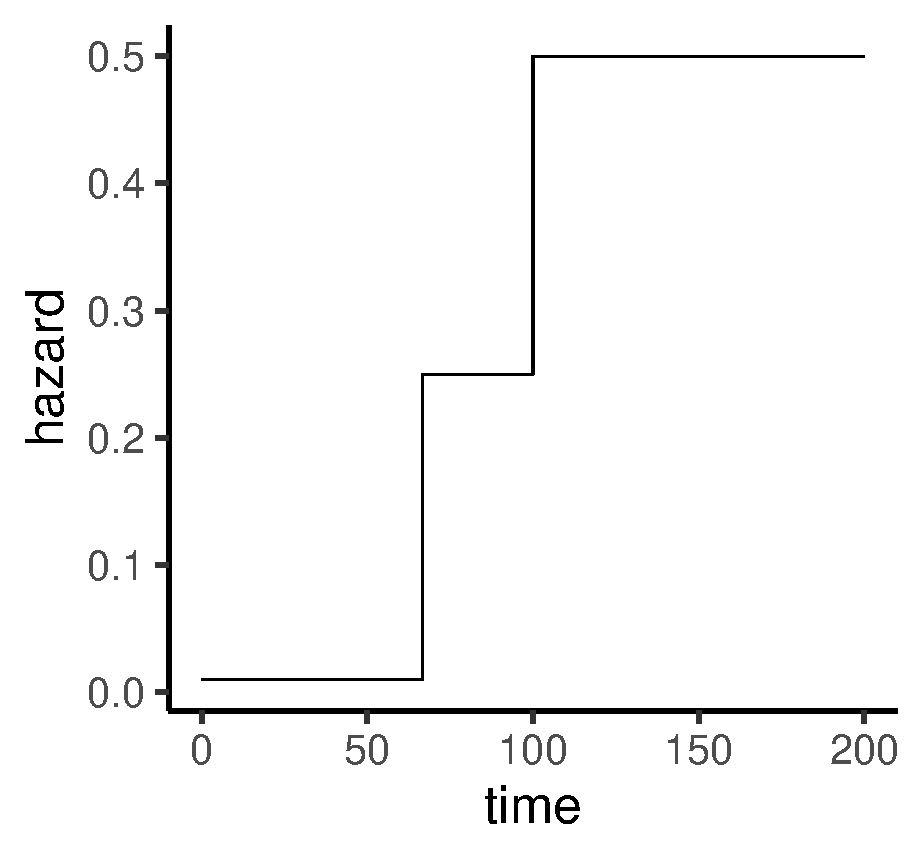
\includegraphics[width=0.55\textwidth,height=2.5in]{base_sim1.pdf}
\caption{True Baseline Hazard in the first example in \ref{subsubsec:sim1}.}
\label{fig:truebase1}
\end{figure}


\begin{figure}[ht]
\centering
\subfigure[Simple stepwise baseline]{
  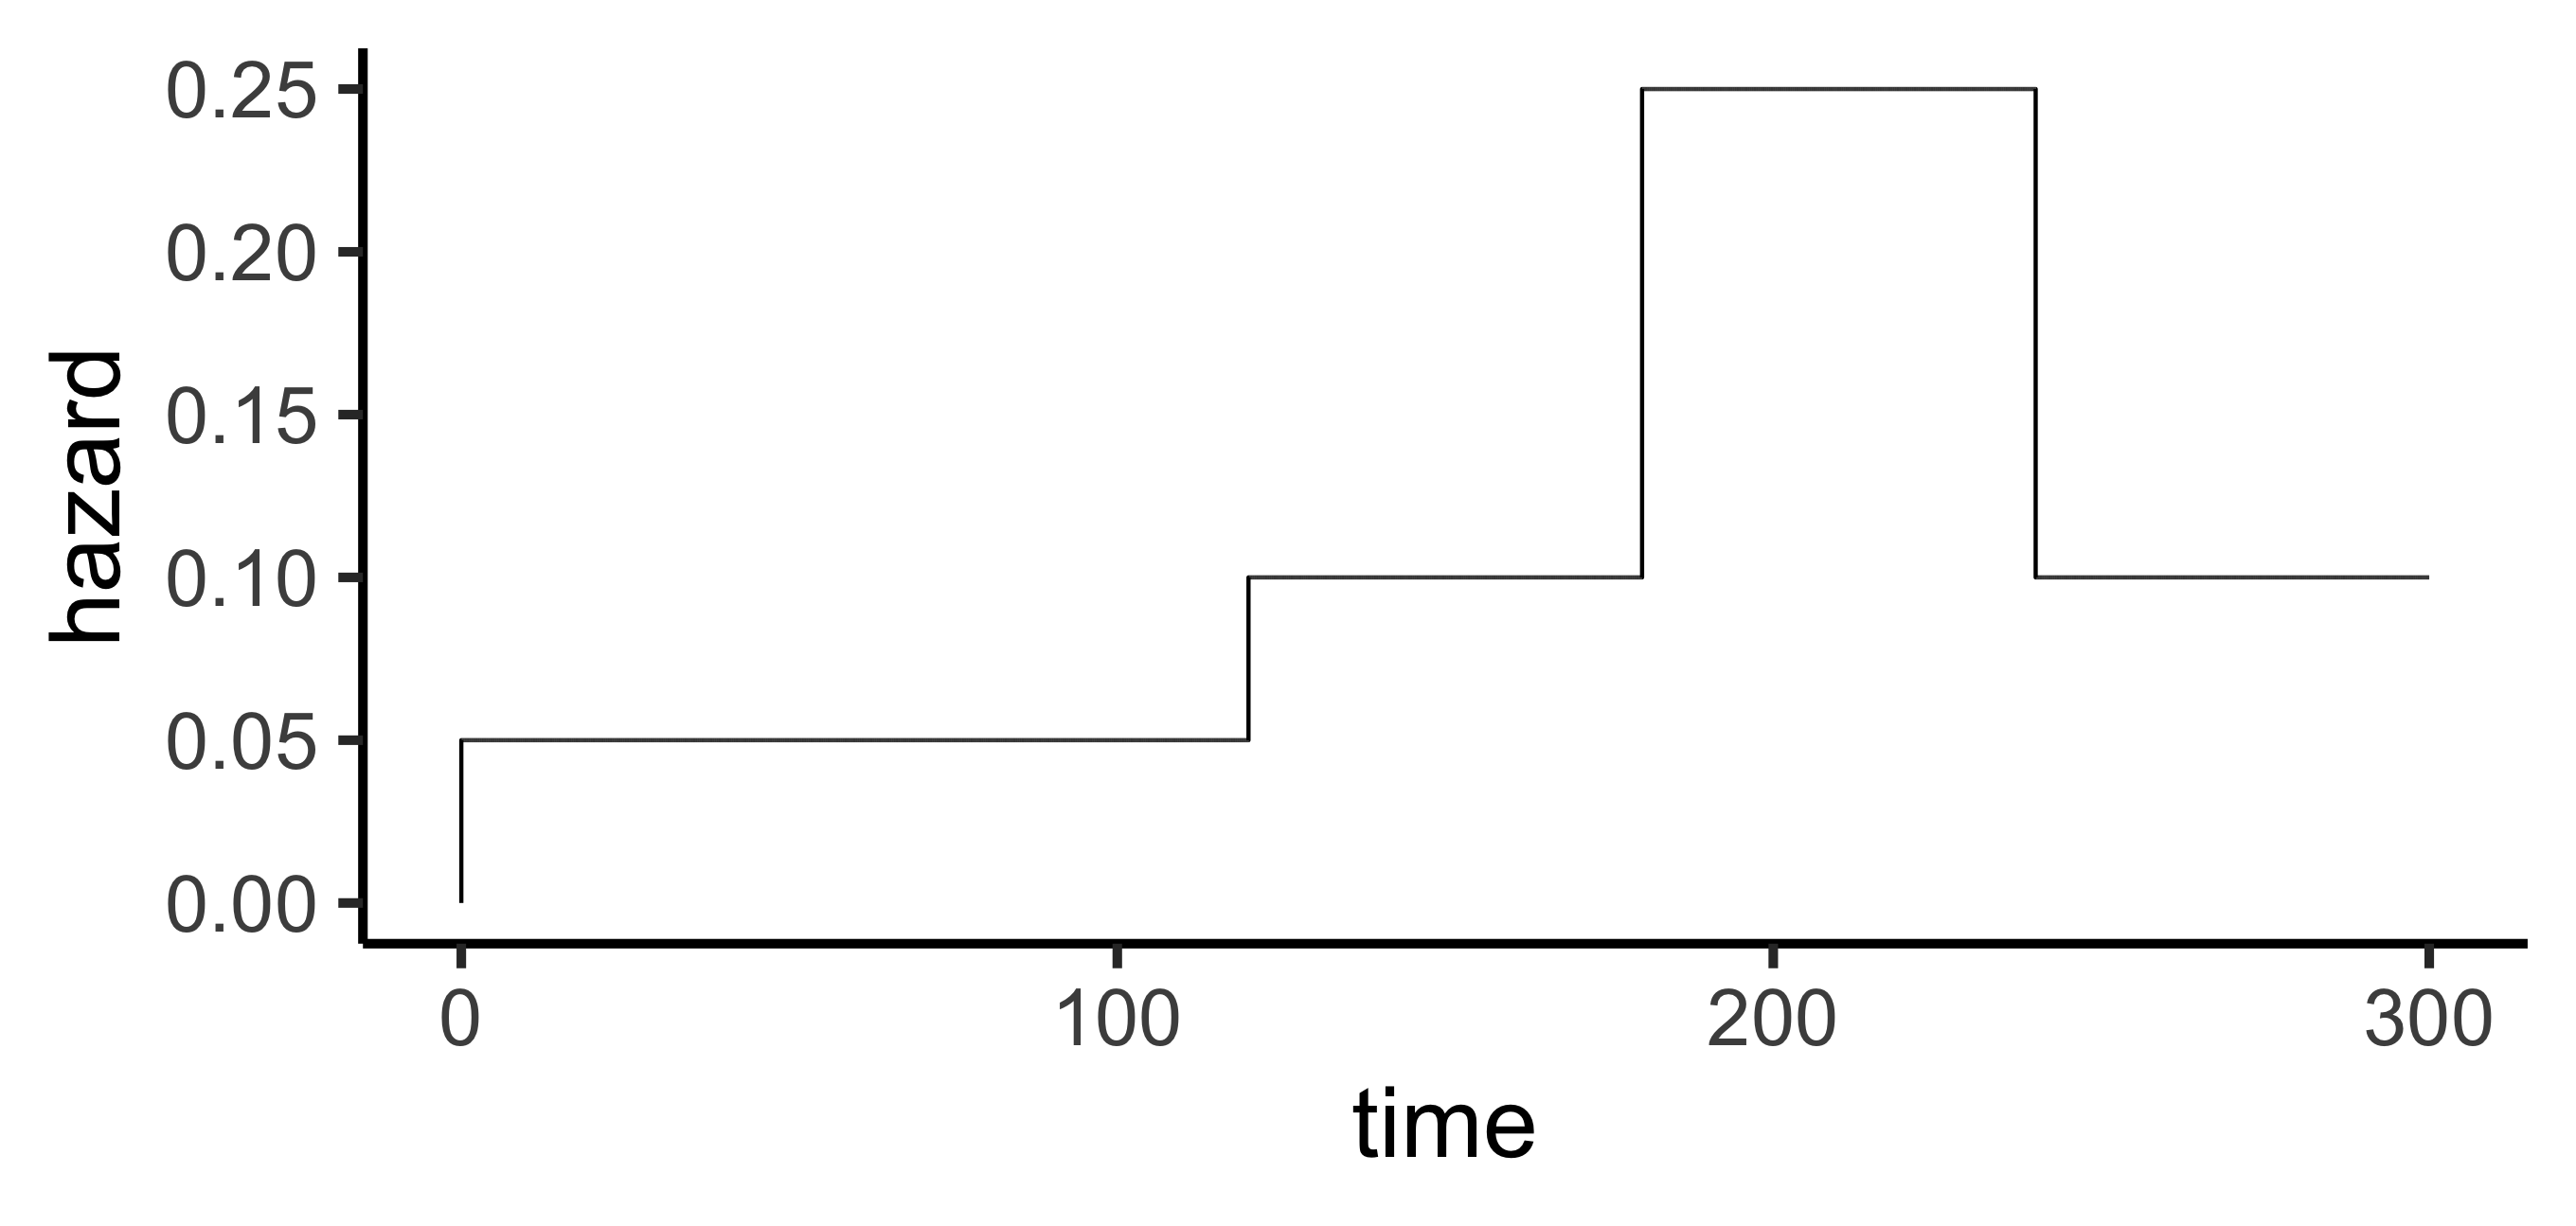
\includegraphics[width=0.45\textwidth,height=2.5in]{simple_base.png}
}
\subfigure[Oscillating stepwise baseline]{
  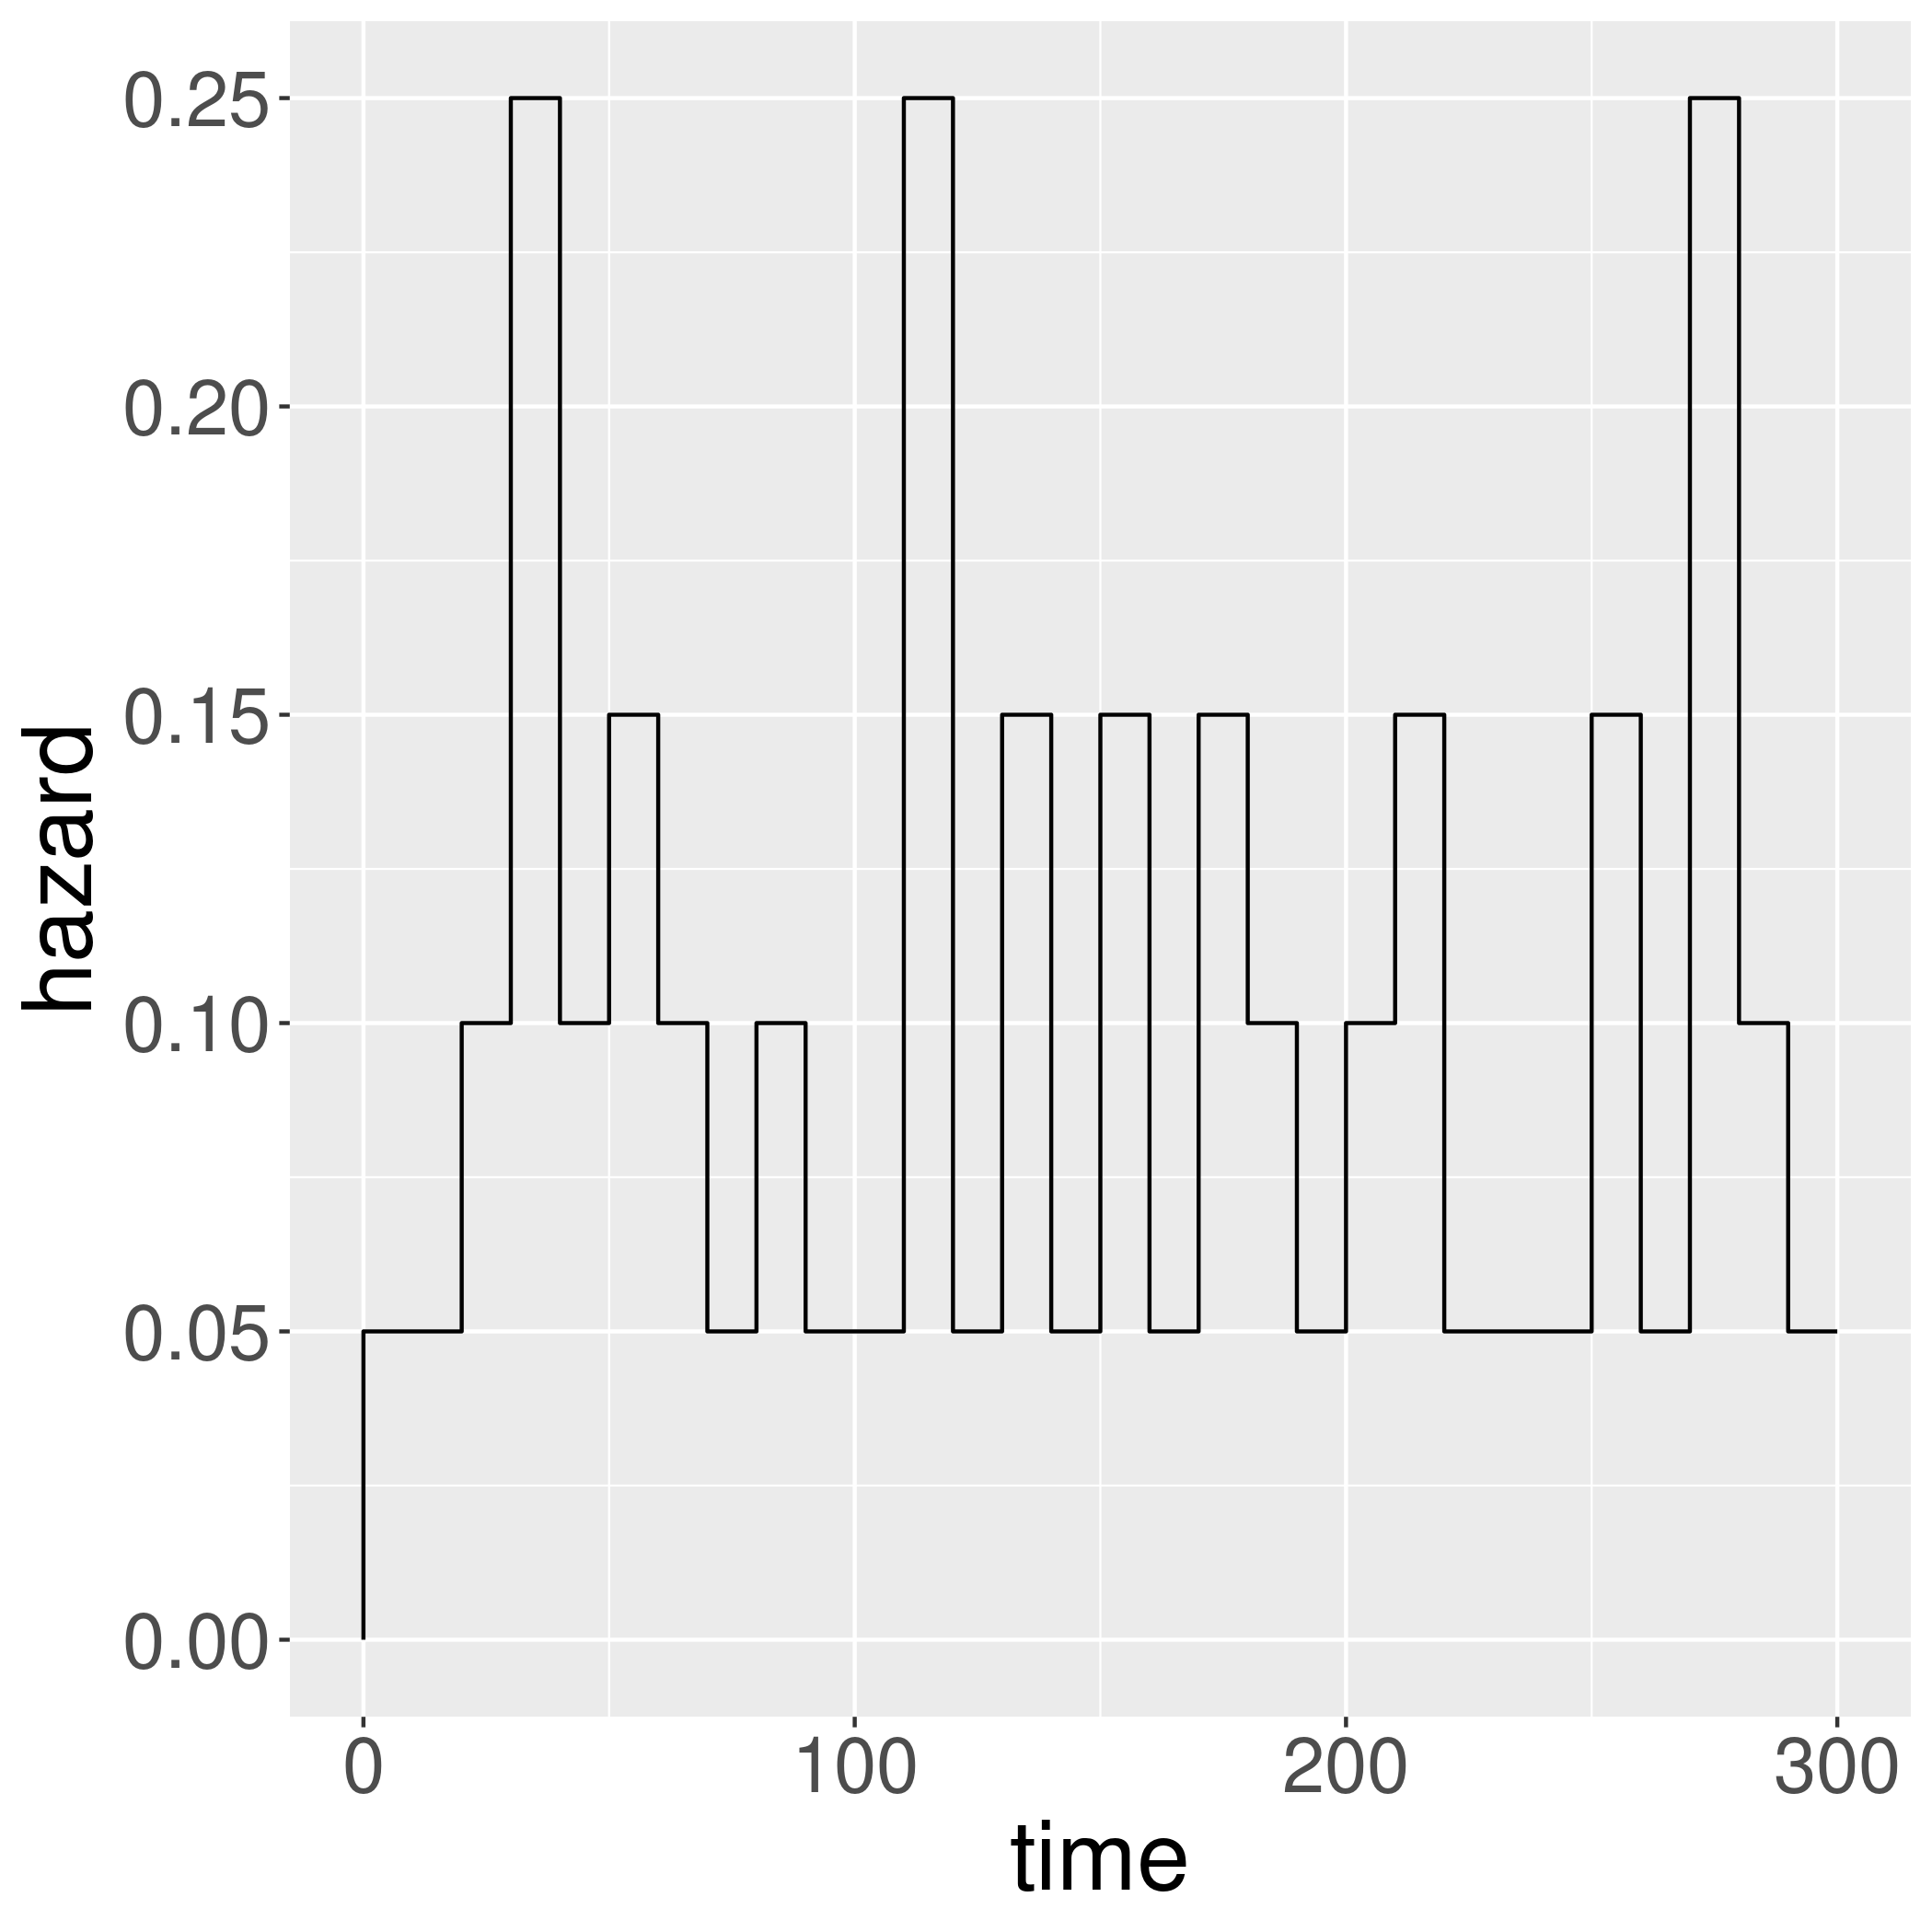
\includegraphics[width=0.45\textwidth,height=2.5in]{stepwise_base.png}
}
\subfigure[Complicated baseline]{
	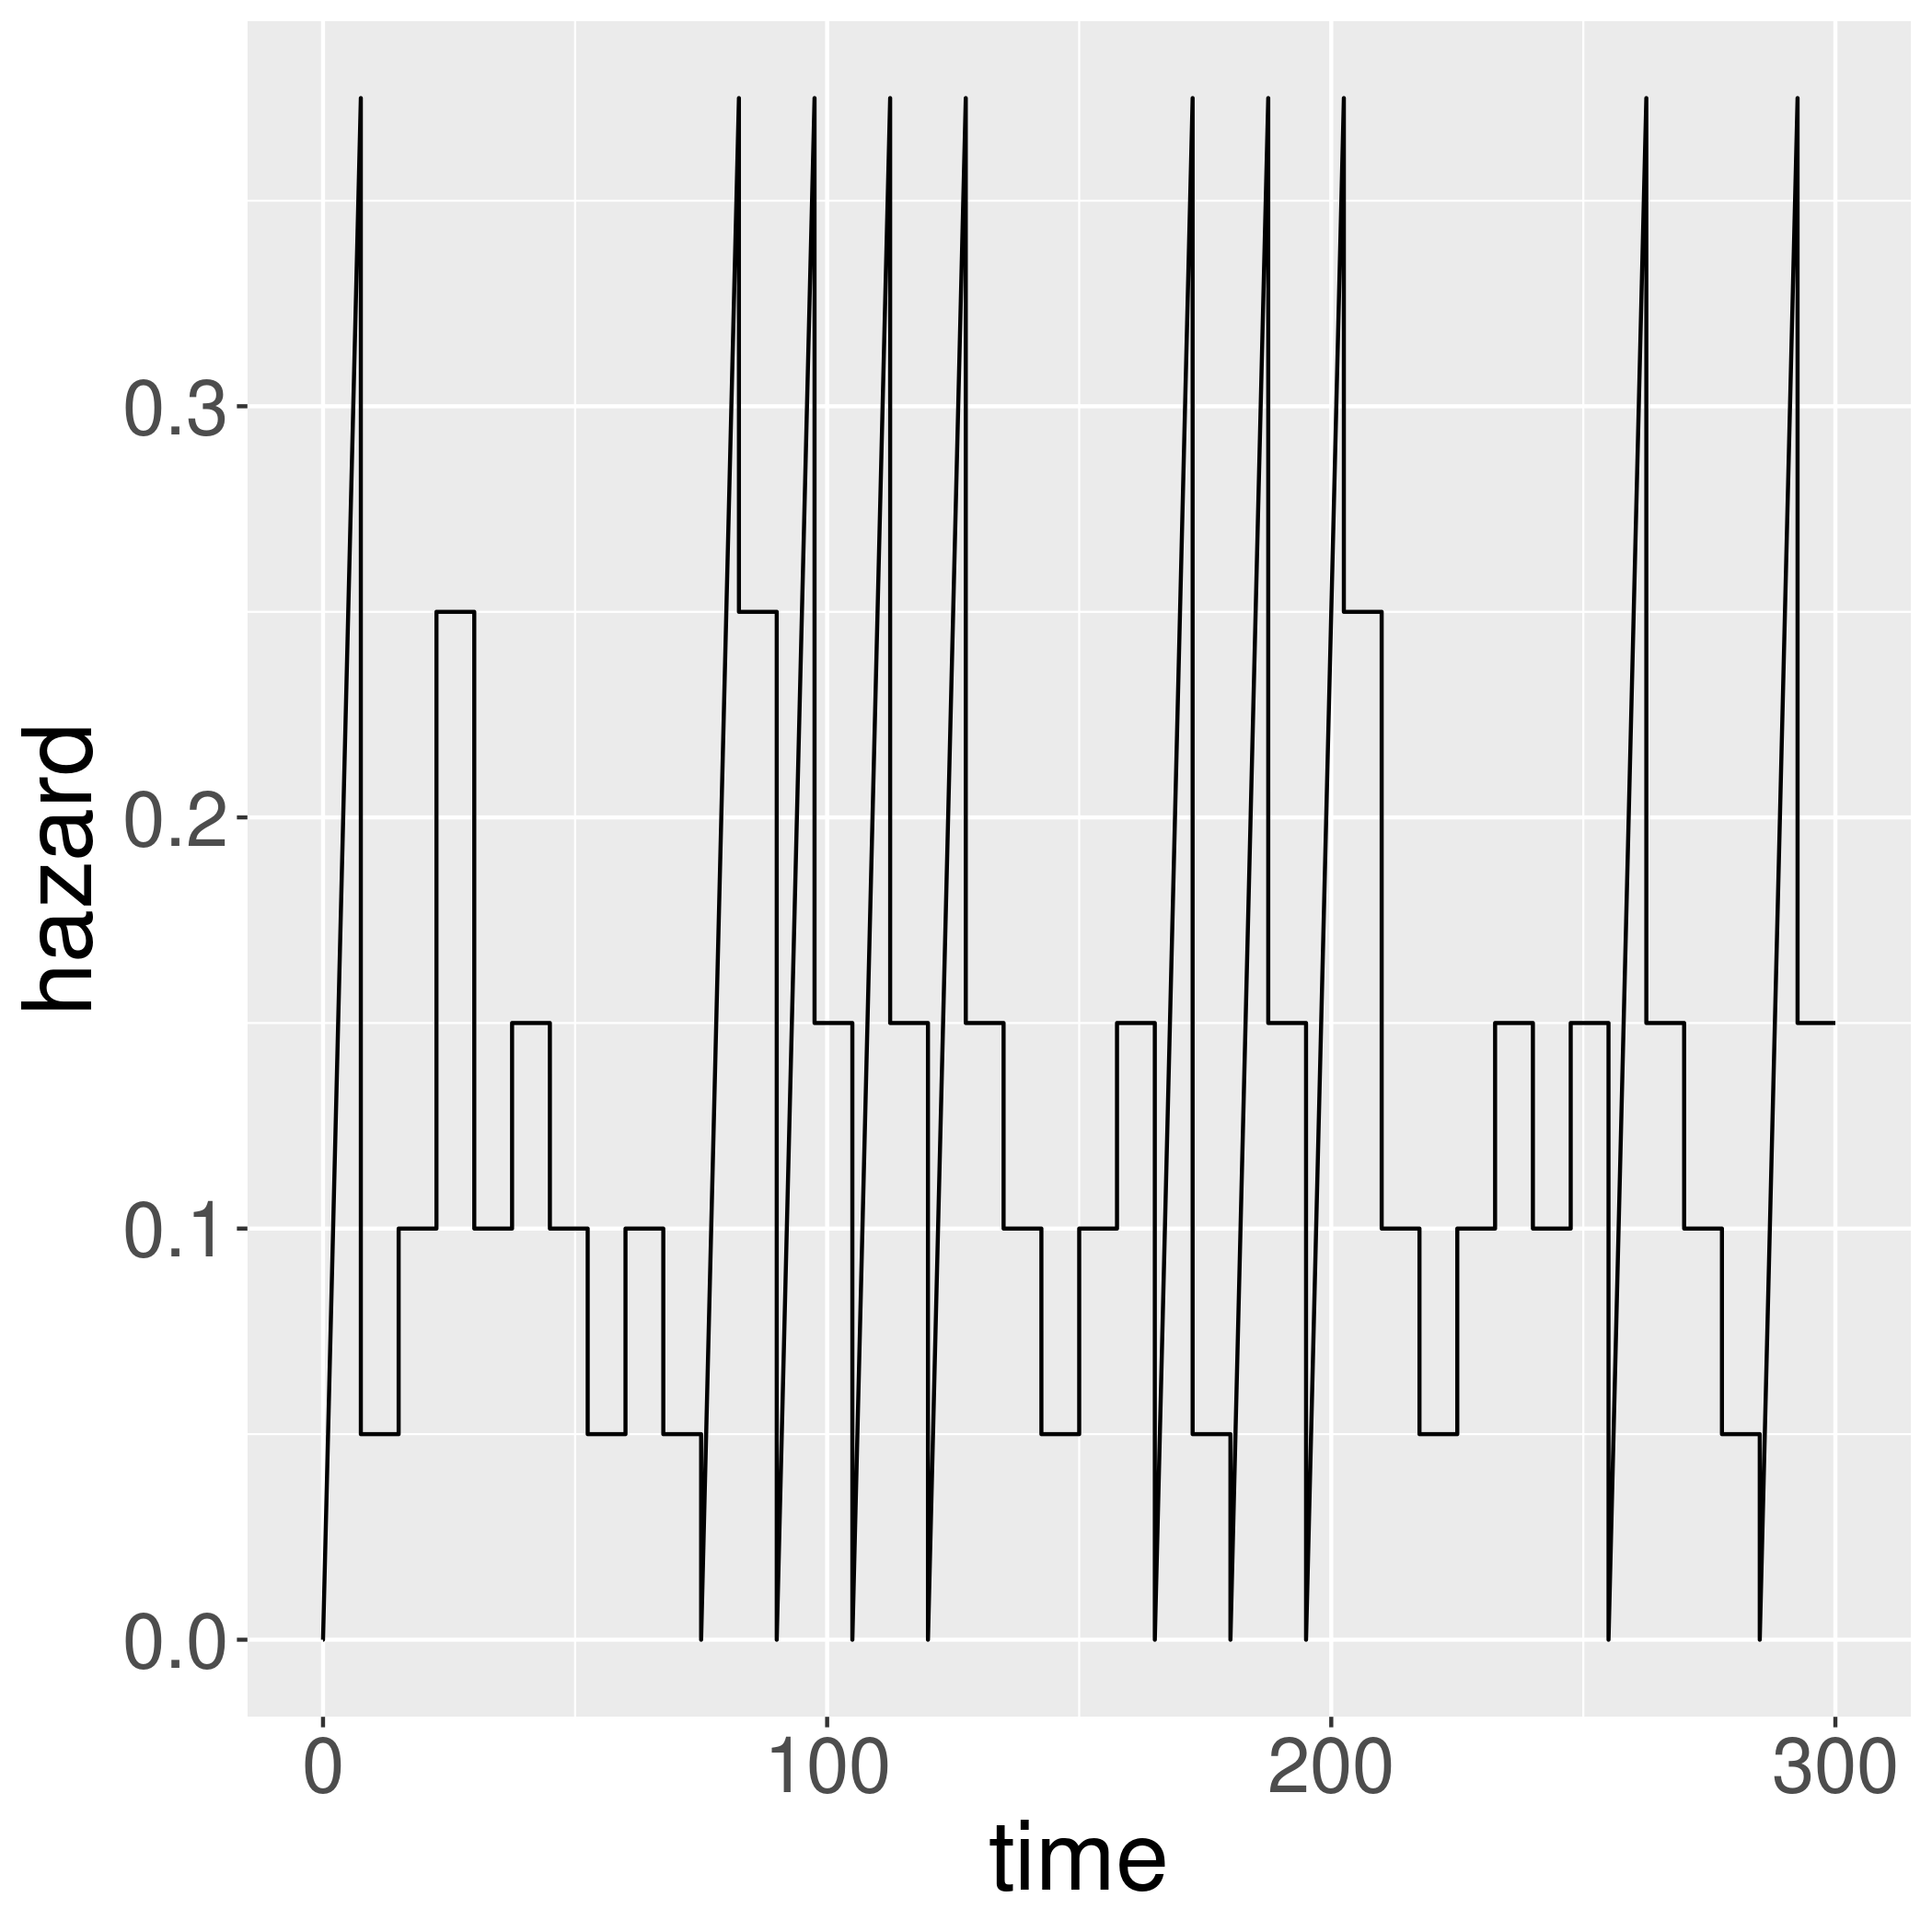
\includegraphics[width=0.55\textwidth,height=2.5in]{com_base.png}
}
\caption{True Baseline Hazards in the second example in \ref{subsubsec:sim2}.}
\label{fig:truebase2}
\end{figure}


\begin{figure}[ht]
\centering
\subfigure[Simple stepwise baseline]{
  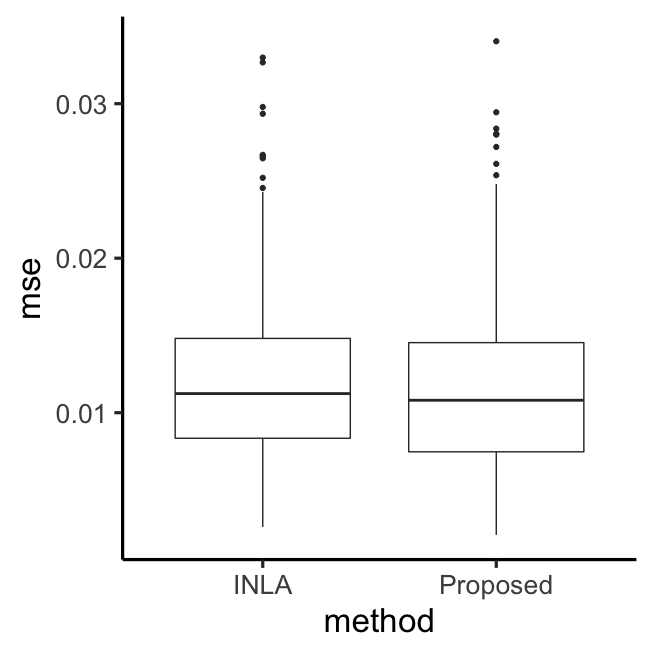
\includegraphics[width=0.45\textwidth,height=2.5in]{simple_box.png}
}
\subfigure[Oscillating stepwise baseline]{
  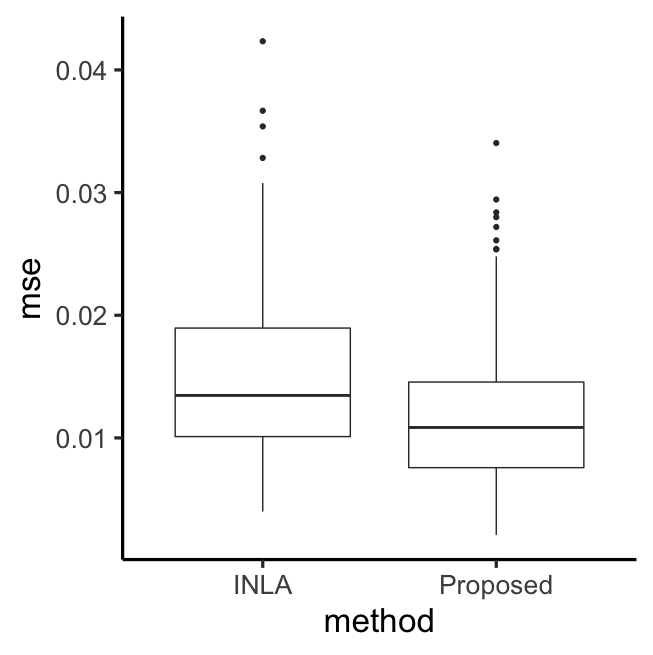
\includegraphics[width=0.45\textwidth,height=2.5in]{stepwise_box.png}
}
\subfigure[Complicated baseline]{
	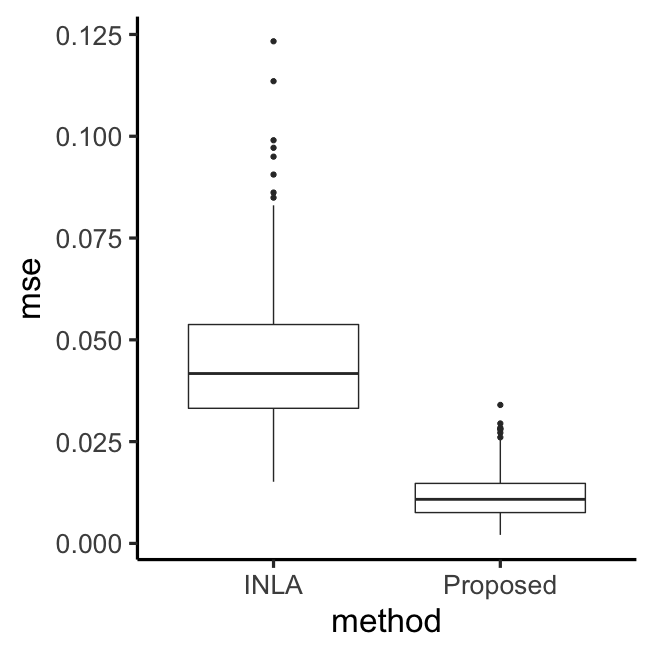
\includegraphics[width=0.55\textwidth,height=2.5in]{com_box.png}
}
\caption{Results for the second simulation in section \ref{subsubsec:sim2}. (a): Box-plot of MSE from 300 replications with simple baseline, using INLA and the proposed method. (b): Box-plot of MSE from 300 replications with oscillating baseline, using INLA and the proposed method. (c): Box-plot of MSE from 300 replications with complicated baseline, using INLA and the proposed method.}
\label{fig:SimAggBox}
\end{figure}



\begin{table}
\begin{center}
\scalebox{0.8}{
\begin{tabular}{||c c c c c||}
 \hline
 Baseline Hazards & $\xi$ Coverage Rate (Proposed) & $\xi$ Coverage Rate (INLA) & $\xi$ MSE (Proposed)& $\xi$ MSE (INLA)\\
 \hline\hline
 Simple Baseline & 0.969 & 0.974 & 0.0116 & 0.0122 \\
 \hline
Oscillating Baseline  & 0.968 & 0.949 & 0.0117 & 0.0148 \\
 \hline
Complicated Baseline & 0.968 & 0.659 & 0.0117 & 0.0448 \\
  \hline \hline
\end{tabular}
}
\end{center}
\caption{Comparison metrics in terms of MSE and posterior coverage rate from 300 independent replications, for the three baselines in the second simulation study in section \ref{subsubsec:sim2}.}
\label{table:Sim2Agg}
\end{table}






\begin{figure}[ht]
\centering
\subfigure[Posterior effect of \texttt{tpi}]{
  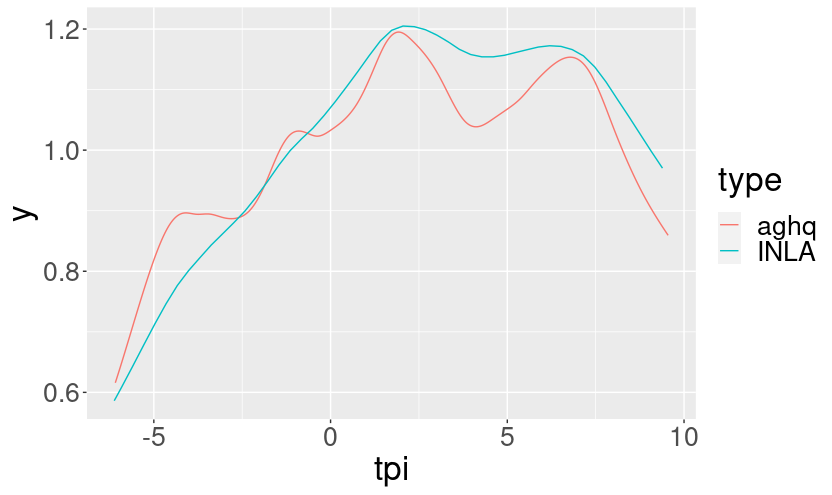
\includegraphics[width=0.45\textwidth,height=2.5in]{leukSmooth.png}
}
\subfigure[Posterior distribution of $\sigma$]{
  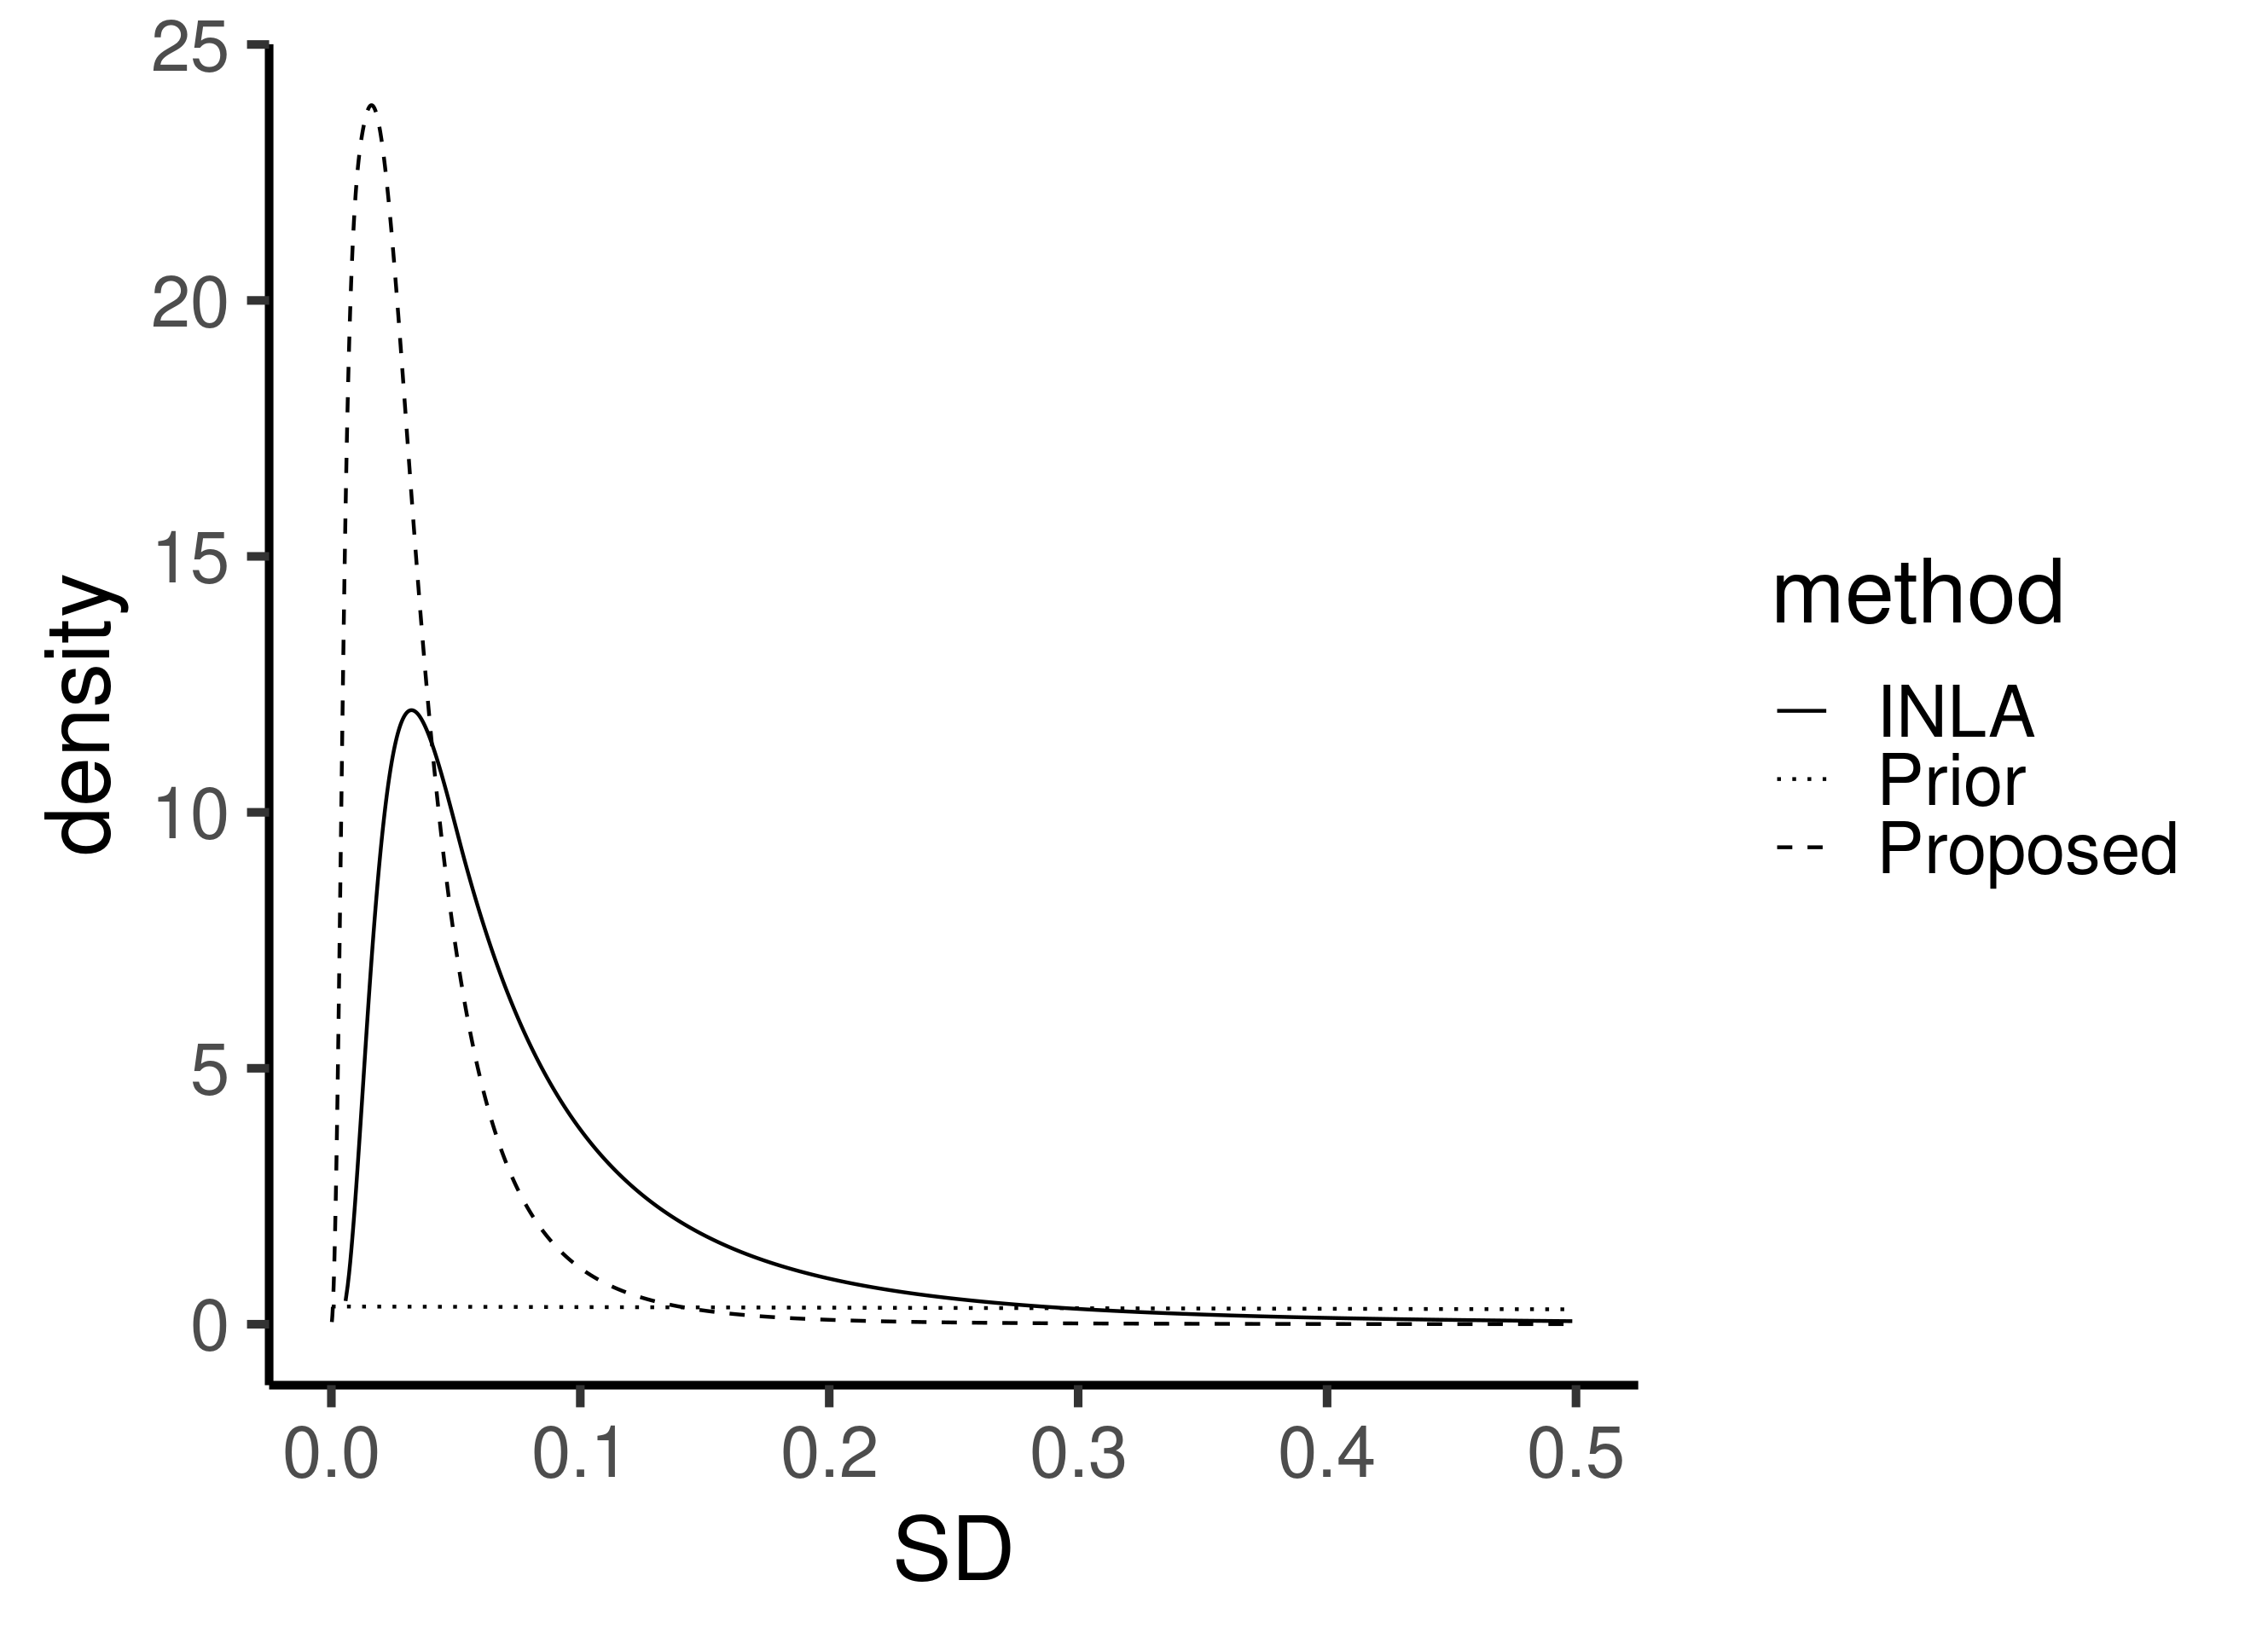
\includegraphics[width=0.45\textwidth,height=2.5in]{leukHyper.png}
}
\subfigure[Posterior distributions of $\sigma$]{
  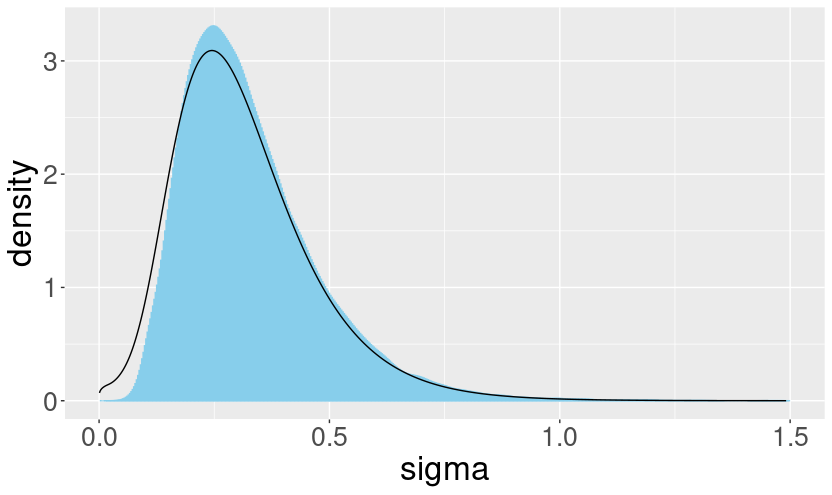
\includegraphics[width=0.55\textwidth,height=2.5in]{leukHyper2.png}
}
\caption{Results for the Leukemia data in section \ref{subsec:leuk}. (a): (Exponentiated) posterior mean for the semi-parametric tpi effect using our proposed method(dashed) and INLA(solid). (b): Prior(dotted) and posterior distributions for $\sigma$ using our proposed method(dashed) and INLA(solid). (c): Posterior distribution for $\sigma$ obtained using MCMC(gray histogram), and using the proposed method(black line).}
\label{fig:leuk}
\end{figure}



\begin{table}
\begin{center}
\scalebox{0.99}{
\begin{tabular}
{|p{3cm}|
p{1cm}|p{1cm}p{1cm}|p{1cm}p{1cm}|}
\hline
\cline{1-6}
      \multicolumn{1}{l}{} &
      \multicolumn{1}{l}{} &
      \multicolumn{2}{c}{Proposed} &
      \multicolumn{2}{c}{INLA}\\
      Variables/Reference & Levels & {Mean} & {SD} & {Mean} & {SD} \\
 \hline
 Age & & 0.00467 & 0.0149 & 0.00235 & 0.0130 \\
 Sex/Male & Female & -1.65  & 0.463  & -1.64 & 0.385 \\
 Disease Type/Other & GN & 0.178 & 0.532 &  0.111 & 0.474 \\
  & AN & 0.420 & 0.528 & 0.519 & 0.467  \\
  & PKD & -1.15 & 0.817  & -1.06 & 0.708 \\
\hline
\end{tabular}
}
\end{center}
\caption{Estimated means and standard deviations of linear effects by proposed method and INLA's full likelihood method for the kidney data in section \ref{subsec:kidney}. }
\label{table:KidneyFixed1}
\end{table}





\begin{table}
\begin{center}
\scalebox{0.99}{
\begin{tabular}
{|p{3cm}|
p{1cm}|p{1cm}p{1cm}|p{1cm}p{1cm}|}
\hline
\cline{1-6}
      \multicolumn{1}{l}{} &
      \multicolumn{1}{l}{} &
      \multicolumn{2}{c}{Proposed} &
      \multicolumn{2}{c}{MCMC}\\
      Variables/Reference & Levels & {Mean} & {SD} & {Mean} & {SD} \\
 \hline
 Age & & 0.00467 & 0.0149 & 0.00516 & 0.0158 \\
 Sex/Male & Female & -1.65  & 0.463  & -1.72 & 0.507 \\
 Disease Type/Other & GN & 0.178 & 0.532 &  0.172 & 0.576 \\
  & AN & 0.420 & 0.528 & 0.415 & 0.573  \\
  & PKD & -1.15 & 0.817  & -1.26 & 0.859 \\
\hline
\end{tabular}
}
\end{center}
\caption{Estimated means and standard deviations of linear effects by proposed method and MCMC method for the kidney data in section \ref{subsec:kidney}. }
\label{table:KidneyFixed2}
\end{table}




\begin{figure}[ht]
\centering
\subfigure[Posterior distributions of $\sigma$]{
  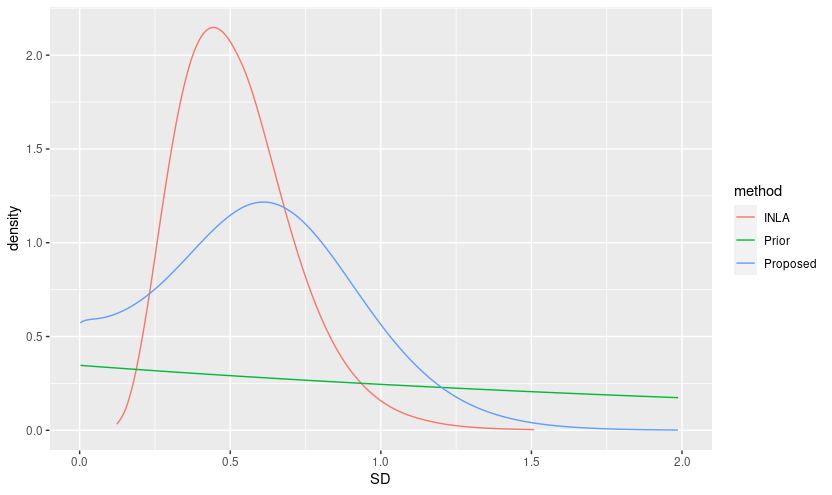
\includegraphics[width=0.45\textwidth,height=2.5in]{kidneyHyper.png}
}
\subfigure[Posterior distributions of $\sigma$]{
  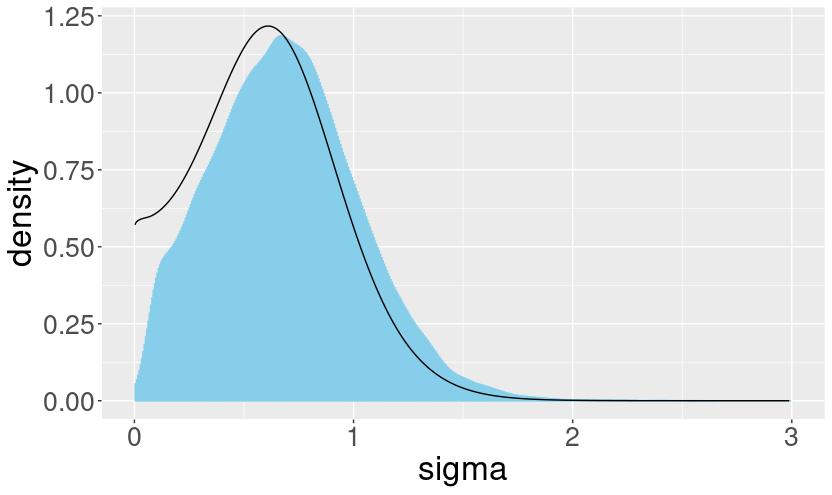
\includegraphics[width=0.45\textwidth,height=2.5in]{kidneyHyper2.png}
}
\caption{Results for the kidney data in section \ref{subsec:kidney}. (a): Prior(dotted) and posterior distributions for $\sigma$ using our proposed method(dashed) and INLA(solid) (b): Posterior distribution for $\sigma$ obtained using MCMC(gray histogram), and using the proposed method(black line).}
\label{fig:kidneyHyper}
\end{figure}





\end{document}

